\section{Additional Applications of the Learned Change of Variables}\label{sec:apx:additional_applications}

The experiments from the main text use the trained encoder and flow as a learned, nonlinear change of variables in order to precondition the voxelwise posterior sampling problem.
The same change of variables can be used to accelerate related optimization and sampling problems without retraining.
This section illustrates three example use cases.

\subsection{\texorpdfstring{\gls*{ELBO}}{ELBO}-Based Flip-Angle Estimation}\label{sec:apx:flip_angle_elbo}

The \gls*{EPG} basis matrix depends on the sequence of excitation and flip angles $\alpha_{\mathrm{ex}}, \alpha_1, \ldots, \alpha_{n_{\TE}}$.
As detailed in \cref{sec:apx:epg_basis}, the ideal \gls*{CPMG} sequence of flip angles $\pi/2, \pi, \ldots$ is perturbed by $B_1$ inhomogeneity.
This is modelled by a voxelwise effective flip angle $\alpha$ where $\alpha_{\mathrm{ex}} = \alpha / 2$ and $\alpha_j = \alpha$.
In the main experiments, $\alpha$ is fixed per voxel, estimated by \gls*{DECAES} preprocessing, which finds the $\alpha$ which minimizes the \gls*{NNLS} residual norm $\hat{\alpha}_{\mathrm{DECAES}} = \argmin_{\alpha} \min_{x \ge 0} \lVert A(\alpha) x - \signal \rVert_2$.
Instead, using the trained encoder, flow, and prior, we can optimize $\alpha$ directly against a variational objective.
In our application, $\alpha$ varies over the voxels of a 3D brain volume;
we investigate two representations:
as an array of independent voxelwise values $\alpha_{ijk}$, or as a low-order polynomial field $\alpha(x, y, z) = \sum_{0 \leq a + b + c \leq K} w_{abc} x^a y^b z^c$.

Each estimate of $\alpha$ affects $A(\alpha)$, which is used both in the likelihood and implicitly through the flow $\varphi(\cdot; z(\alpha))$ via the encoder conditioning vector $z(\alpha)$,
\begin{align}
    z(\alpha) = \enc(\signal, A(\alpha), \theta(\alpha)),
\end{align}
where $\theta(\alpha)$ is the scalar feature vector from~\eqref{eqn:scalar_features}.
We aim to avoid differentiating through $z(\alpha)$, since backpropagating through the encoder at every iteration would dominate per-step costs;
instead, we hold $z(\alpha)$ fixed at the \gls*{DECAES} estimate $z(\hat{\alpha}_{\mathrm{DECAES}})$ in the objectives below, refreshing intermittently outside of gradient computations only if needed.
We consider three optimization objectives of increasing computational cost and statistical robustness, as well as a Bayesian sampling method.

The simplest estimate, and closest in spirit to \gls*{DECAES}, is a maximum a posteriori (\gls*{MAP}) estimate.
A full \gls*{MAP} estimate jointly minimizes the negative log posterior over $(\vv{u}, \alpha)$,
\begin{align}\label{eqn:apx:flip_angle_full_map}
    \mathcal{M}(\vv{u}, \alpha) & = -\log p(\signal \mid \varphi(\vv{u}; z(\alpha)), A(\alpha)) \nonumber \\
                                & \quad -\log p(\varphi(\vv{u}; z(\alpha))) \nonumber                     \\
                                & \quad -\log \left| \det J_\varphi(\vv{u}; z(\alpha)) \right|.
\end{align}
The trained flow acts only as a nonlinear change of variables, making the problem easy to solve from the initial guesses $\vv{u} = 0$ and $\alpha = \hat{\alpha}_{\mathrm{DECAES}}$.

An even cheaper estimate fixes the \textit{pseudo-mode} $\vv{u} = \Zero$ -- which a well-trained $\varphi$ maps close to the true posterior mode for any given $z(\alpha)$ -- and minimizes the pseudo-\gls*{MAP} objective
\begin{align}\label{eqn:apx:flip_angle_pseudo_map}
    \mathcal{L}(\alpha) & = -\log p(\signal \mid \bar{\distbn}_0, \eta_0, A(\alpha)) \nonumber \\
                        & \quad -\log p(\bar{\distbn}_0, \eta_0),                              \\
                        & \text{where} \quad
    \bar{\distbn}_0, \eta_0 = \varphi(\Zero; z(\alpha)), \nonumber
\end{align}
where $\bar{\distbn}_0$ is the marginal pseudo-mode of the $T_2$ distribution, and $\eta_0 = (\log s, \log \sigma)$ are the nuisance parameters.
With $z(\alpha)$ fixed, $\bar{\distbn}_0$ does not depend on $\alpha$ and can be precomputed.
The nuisance mode $\eta_0(\alpha)$ must be recomputed at each step, since its value is the Laplace mode~\eqref{eqn:laplace_mean} of the conditional posterior given the forward signal $A(\alpha) \bar{\distbn}_0$;
this is comparatively cheap, as it reuses the Newton solver of \cref{subsubsec:laplace_approximation} and the implicit-function gradients~\eqref{eqn:implicit_gradients}.
The pseudo-\gls*{MAP} relies more heavily on the quality of the variational posterior since it assumes that the marginal pseudo-mode $\bar{\distbn}_0$ is a good enough approximation to the true \gls*{MAP} estimate, but it is much cheaper to compute and, as we will see, produces visually indistinguishable flip angles.

Both of these point estimates ignore the spread of the posterior over $\vv{u}$.
To account for this, $\alpha$ may instead be chosen to minimize the free energy
\begin{align}\label{eqn:apx:flip_angle_elbo}
    \mathcal{F}(\alpha) & = \mathbb{E}_{u \sim \pi_{\vv{u}}} \Bigl[ -\log p(\signal \mid \varphi(u; z(\alpha)), A(\alpha)) \nonumber \\
                        & - \log p(\varphi(u; z(\alpha))) + \log q(\varphi(u; z(\alpha)) \mid \signal, A(\alpha)) \Bigr],
\end{align}
with the trained flow held fixed.
Since $\mathcal{F}(\alpha)$ is the negative evidence lower bound, minimizing it maximizes a variational lower bound on the marginal log-evidence $\log p(\signal \mid \alpha)$; the encoder is refreshed as $\alpha$ changes.
The free energy averages over the approximate posterior rather than using a single mode, and is correspondingly more expensive.
All point estimates are initialized from the \gls*{DECAES} estimate $\hat{\alpha}_{ijk}$, and the polynomial field from the linear least-squares fit $\argmin_{\alpha} \sum_{ijk} (\alpha(x_i, y_j, z_k) - \hat{\alpha}_{ijk})^2$.
The deterministic \gls*{MAP} objectives and the stochastic free-energy objective are minimized by \textsc{PSGD} with Newton-type preconditioners fitted to Hessian-vector products~\citep{li_preconditioned_2018}.
Note that the polynomial field is spatially coupled, so each coefficient is informed by many voxels and a single Monte Carlo sample of $\vv{u}$ gives a stable descent direction, whereas with one flip angle per voxel the gradients have more variance and several samples must be averaged per iteration to suppress the sampling noise.

Minimizing $\mathcal{F}(\alpha)$ still yields only a variational evidence point estimate of $\alpha$.
To quantify the uncertainty in the $\alpha$ estimates, we instead sample from the marginal posterior $p(\alpha \mid \signal) \propto p(\signal \mid \alpha) p(\alpha)$.
There remains the usual complication that the marginal evidence $p(\signal \mid \alpha)$ is intractable, and we can only bound it from below;
however, holding $z(\alpha_{\mathrm{DECAES}})$ fixed, the trained variational posterior allows for an efficient and unbiased estimator
\begin{align}\label{eqn:apx:flip_angle_marginal_estimator}
    \hat{p}(\signal \mid \alpha)
    = \frac{1}{S} \sum_{s=1}^{S} \frac{p(\signal \mid \varphi(u_s; z), A(\alpha))}{q(\varphi(u_s; z) \mid \signal, A(\alpha))} p(\varphi(u_s; z)),
\end{align}
satisfying $\mathbb{E}[\hat{p}(\signal \mid \alpha)] = p(\signal \mid \alpha)$ where $u_s \sim \pi_{\vv{u}}$.
Using this stochastic but unbiased estimate in a sampling routine gives rise to \textit{pseudo-marginal} \gls*{MCMC} (PM-\gls*{MCMC}) methods which, remarkably, preserve the exact marginal posterior $p(\alpha \mid \signal)$~\citep{andrieu_pseudo-marginal_2009}.
That is, given a symmetric proposal distribution, a move from $\alpha$ to $\alpha'$ is accepted with the usual Metropolis--Hastings probability
\begin{align}\label{eqn:apx:flip_angle_pmmh_accept}
    \min\left\{ 1, \; \frac{\hat{p}(\signal \mid \alpha') p(\alpha')}{\hat{p}(\signal \mid \alpha) p(\alpha)} \right\},
\end{align}
with $\{u_s\}_{s=1}^S$ redrawn for each proposed $\alpha'$.
Empirically, most flip angles are concentrated near the nominal refocusing angle $\pi$.
In order to respect this empirical finding as well as the $2\pi$-periodic and even symmetries of the \gls*{EPG} basis~\eqref{eqn:apx:epg_cosine_series}, we place a von Mises prior $p(\alpha) \propto \exp(\kappa \cos(\alpha - \pi))$ on the flip angle, with mean $\mu = \pi$ fixed and concentration $\kappa$ fit by maximum likelihood to the \gls*{DECAES} estimates $\{\hat{\alpha}_{ijk}\}$.

\begin{figure*}[th]
    \centering
    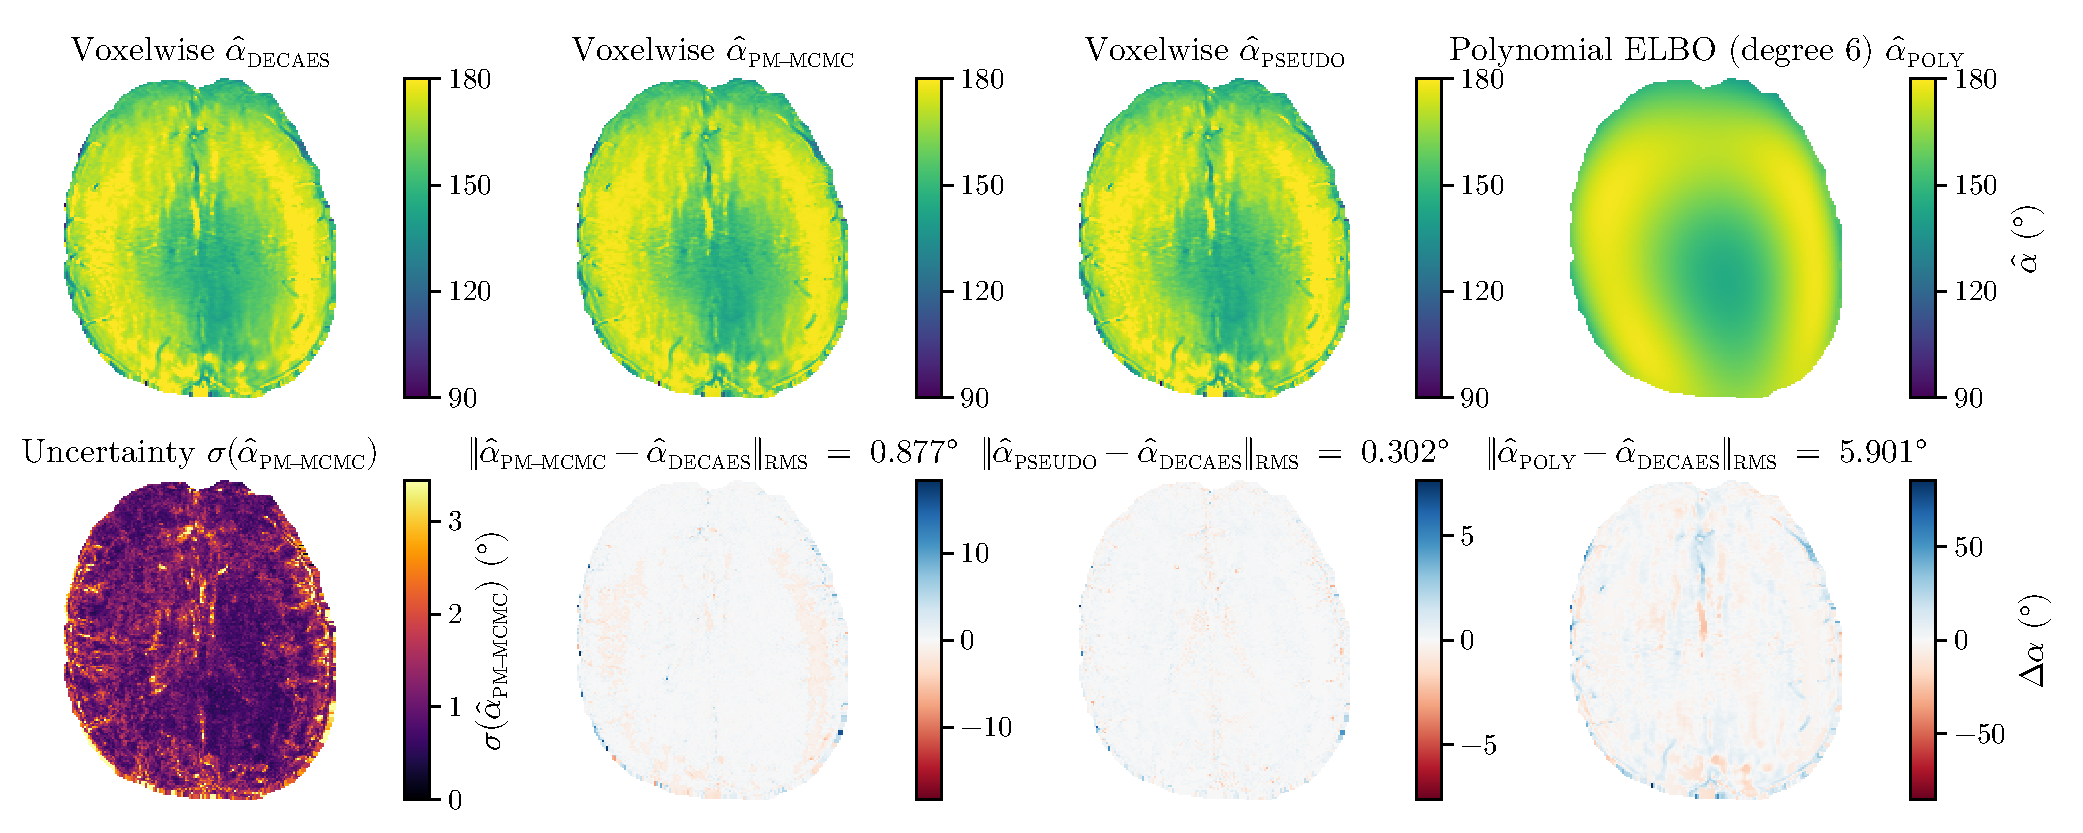
\includegraphics[width=\linewidth]{figures/flip_angle_elbo_comparison.pdf}
    \caption{Flip-angle estimation using the pre-trained flow, optimizing $\alpha$ through its effect on the \gls*{EPG} basis matrix. Top row: the \gls*{DECAES} flip-angle map, the voxelwise PM-\gls*{MCMC} posterior median~\eqref{eqn:apx:flip_angle_marginal_estimator}, the voxelwise pseudo-\gls*{MAP} estimate~\eqref{eqn:apx:flip_angle_pseudo_map}, and a degree-6 polynomial free-energy estimate~\eqref{eqn:apx:flip_angle_elbo}. Bottom row: the voxelwise standard deviation of the PM-\gls*{MCMC} posterior samples, folded onto $[0, \pi]$, and the pointwise difference between the top-row estimate and the \gls*{DECAES} estimate.}
    \label{fig:flip_angle_elbo_comparison}
\end{figure*}

\begin{figure*}[th]
    \centering
    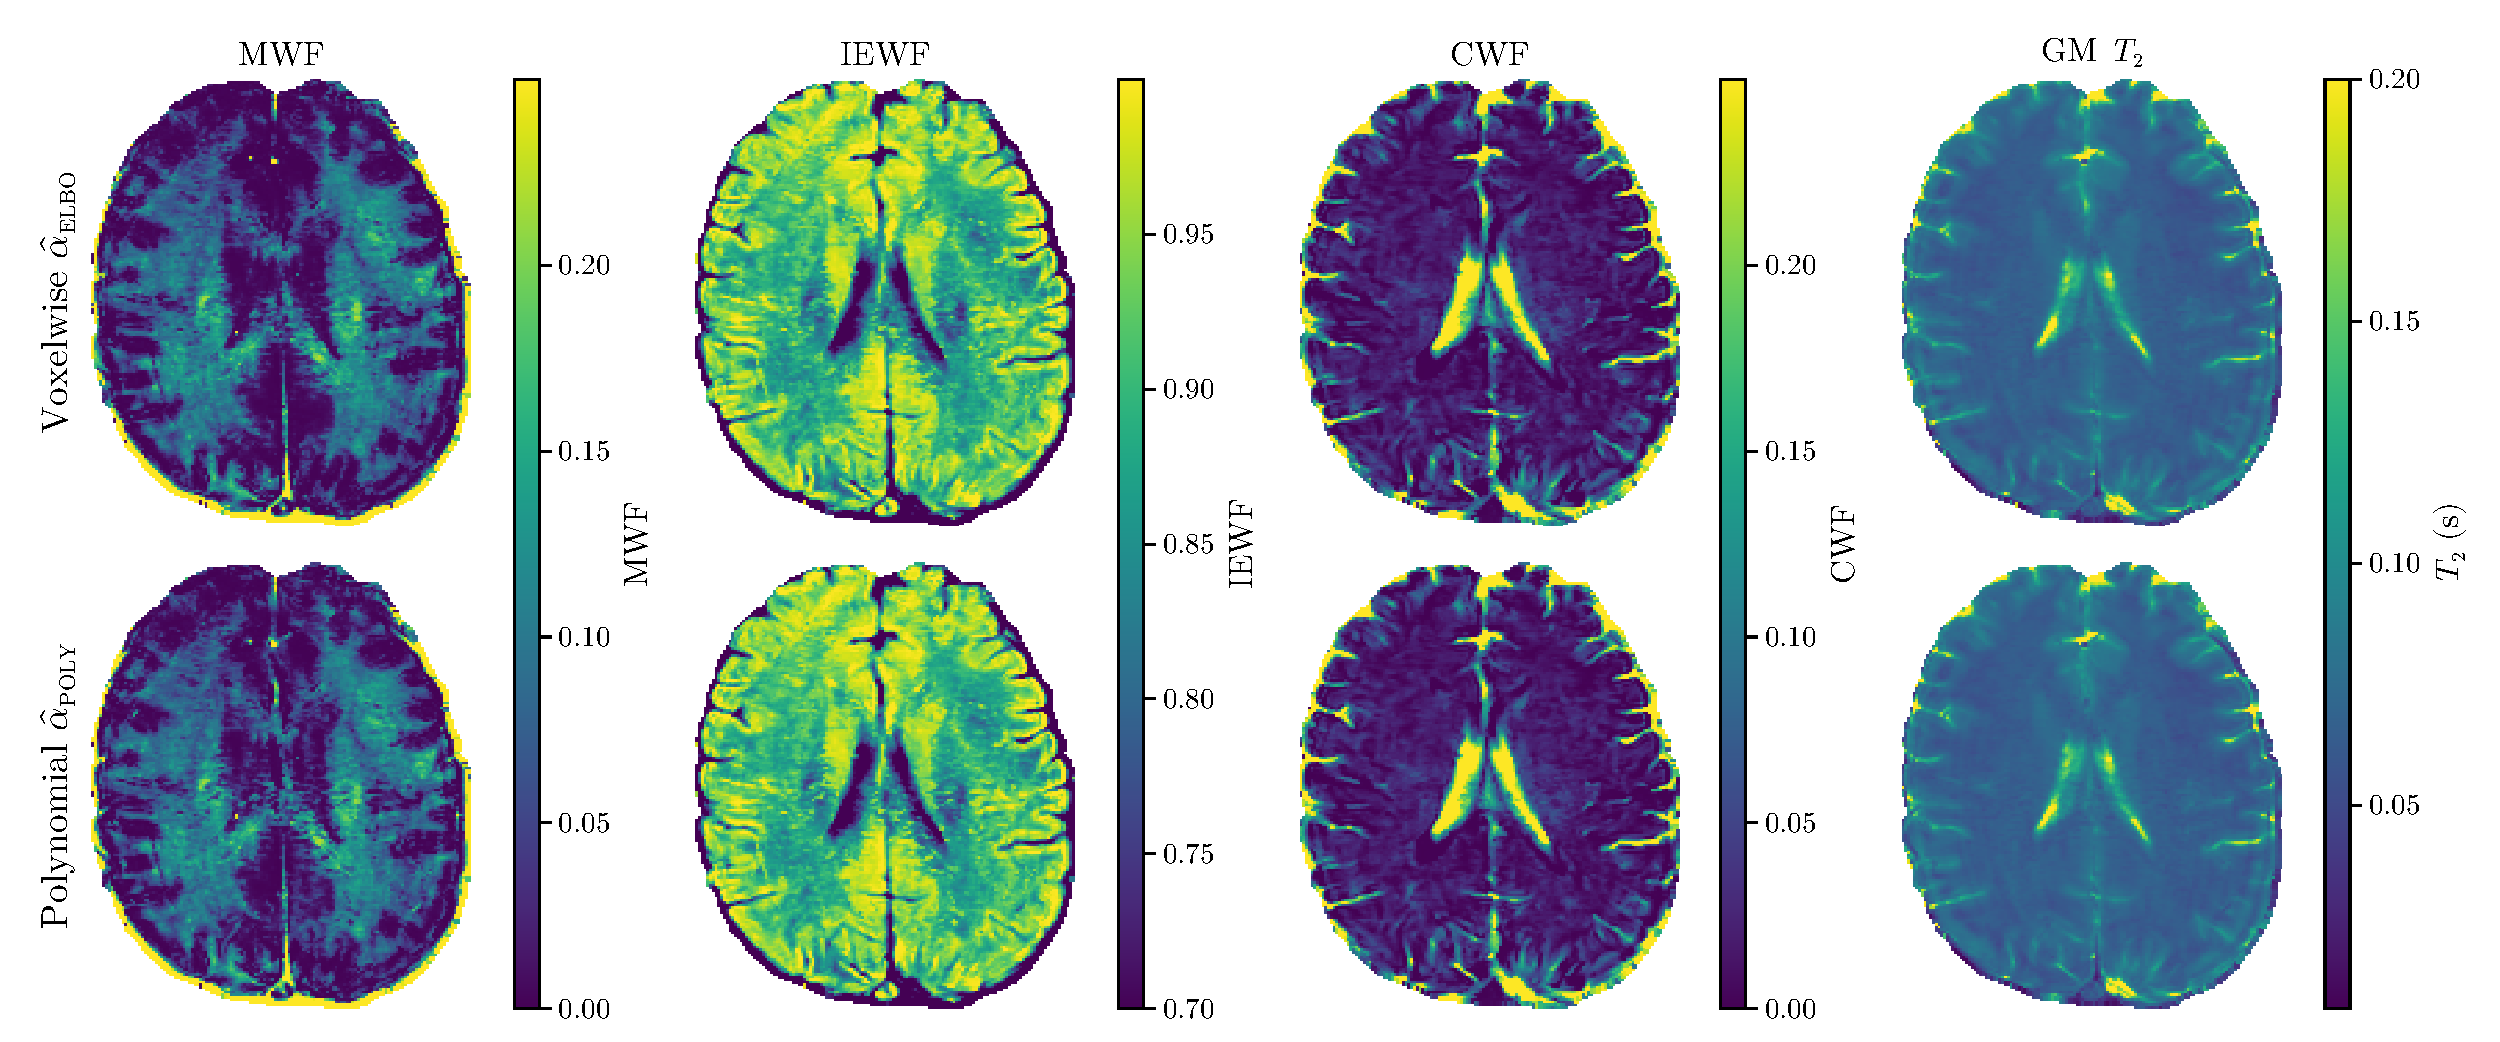
\includegraphics[width=\linewidth]{figures/flip_angle_observables.pdf}
    \caption{Biomarker maps using free-energy minimizing flip-angle estimates. Columns show the myelin water fraction, intra-/extracellular water fraction, cerebrospinal-fluid water fraction, and geometric-mean $T_2$, each computed via independent-proposal Metropolis--Hastings sampling with the pre-trained flow model. Top row: voxelwise flip-angle estimate~\eqref{eqn:apx:flip_angle_elbo}. Bottom row: degree-6 polynomial estimate. The two flip-angle maps differ by a few degrees for typical voxels; the corresponding derived biomarkers agree closely, with one exception: the myelin water fraction appears spuriously underestimated using the polynomial flip-angle map.}
    \label{fig:flip_angle_observables}
\end{figure*}

\begin{table}[htbp]
    \centering
    \begin{tabular}{cccc}
  \toprule
  \textbf{$\text{Method}$} & \textbf{$\text{DECAES}$} & \textbf{$\text{PM-MCMC}$} & \textbf{$\text{Pseudo-mode}$} \\
  \midrule
  PM-MCMC                  & $0.32^{2.0}_{0.015}$     & ---                       & ---                           \\
  Pseudo-mode              & $0.13^{0.75}_{0.0}$      & $0.22^{1.9}_{0.0095}$     & ---                           \\
  Polynomial               & $2.6^{16.0}_{0.13}$      & $2.4^{16.0}_{0.11}$       & $2.6^{16.0}_{0.12}$           \\
  \bottomrule
\end{tabular}

    \caption{Pairwise median absolute differences $\lvert \hat{\alpha}_i - \hat{\alpha}_j \rvert$ between \gls*{DECAES}, PM-\gls*{MCMC}, pseudo-\gls*{MAP}, and polynomial flip-angle estimates, shown with $2.5$ and $97.5$ percentile values as sub- and superscript.}
    \label{tab:flip_angle_comparison}
\end{table}

Apart from the polynomial field, all flip-angle estimates agree closely.
\Cref{fig:flip_angle_elbo_comparison} compares the \gls*{DECAES} flip-angle map with three representative $\alpha$ estimates:
the voxelwise PM-\gls*{MCMC} posterior median, the voxelwise pseudo-\gls*{MAP}, and the degree $K = 6$ polynomial free-energy minimizer, alongside difference maps of each against \gls*{DECAES}, and the voxelwise posterior standard deviation from the sampler.
\Cref{tab:flip_angle_comparison} reports the median pairwise voxelwise absolute differences alongside 2.5th and 97.5th percentile values.
The voxelwise PM-\gls*{MCMC} and pseudo-mode estimates have median absolute differences from \gls*{DECAES} of $0.32^\circ$ and $0.13^\circ$, respectively, compared with $2.6^\circ$ for the spatially smooth polynomial field.
The close voxelwise agreement indicates that the least-squares \gls*{DECAES} estimate is already robust;
the pseudo-\gls*{MAP} provides a cheap refinement, while the PM-\gls*{MCMC} sampler additionally yields voxelwise posterior uncertainty estimates.
In \cref{fig:flip_angle_elbo_comparison} we see that the flip-angle uncertainty is largest near $\alpha = \pi$;
this is consistent with the \gls*{EPG} basis being constant to first order in $\alpha$ in this region due to symmetry of the algorithm about $\alpha = \pi$, and therefore variations in $\alpha$ have comparatively small effect on the \gls*{EPG} basis.
Because $B_1$ inhomogeneity is expected to vary smoothly and not to follow brain structure, the smooth polynomial field is physically motivated and easy to compute.
Without an independent ground truth we cannot determine whether the smooth or the voxelwise estimate is the more accurate, though in~\cref{fig:flip_angle_observables} we can compare their downstream effect, illustrating the myelin water fraction, geometric-mean $T_2$, and intra-/extracellular water fraction maps computed by independent-proposal \gls*{MH} sampling under the voxelwise and polynomial free-energy flip-angle estimates.

\subsubsection{Cosine Series Representation for Efficient \gls*{EPG} Basis Computation and Differentiation}

As part of minimizing~\cref{eqn:apx:flip_angle_pseudo_map,eqn:apx:flip_angle_elbo}, we must evaluate the \gls*{EPG} basis matrix $A(\alpha)$ and its derivative $\partial A / \partial \alpha$ for many values of $\alpha$ at every step.
Re-running the \gls*{EPG} recursion~\eqref{eqn:mpsv_definition} would be expensive, and the recursion currently has a fast implementation only on the \gls*{CPU}.
This can, however, be avoided by exploiting the algebraic structure of the recursion under a constant refocusing flip angle.
When all refocusing pulses are set to $\alpha$, the rotation matrix~\eqref{eqn:epg_basis_components} is affine in $\cos\alpha$ and $\sin\alpha$ via the half-angle identities $\cos^2(\alpha/2) = (1 + \cos\alpha) / 2$ and $\sin^2(\alpha/2) = (1 - \cos\alpha) / 2$.
Each echo applies one such rotation with interwoven linear $\alpha$-independent relaxation and transition operators.
The transverse magnetization $(\mathbf{M}^{i,j})_1^+$ of~\eqref{eqn:epg_basis_definition} is therefore, having factored out the excitation amplitude $\sin(\alpha/2)$, a real trigonometric polynomial of degree at most $n_{\TE}$ in $\alpha$.
This polynomial is additionally an even function of $\alpha$:
the only $\alpha$-dependence that is odd enters via $\sin\alpha$ factors in the off-diagonal entries of $\vv{R}_{j}$~\eqref{eqn:epg_basis_components} which couple the transverse and longitudinal magnetization;
the remaining entries are even in $\alpha$, and neither the relaxation nor transition matrices mix transverse with longitudinal signal.
Since the \gls*{EPG} algorithm is initialized with purely transverse magnetization, the transfers to and from the longitudinal magnetization occur in pairs, each acquiring a factor of $\sin\alpha$;
every transverse readout echo is therefore even in $\alpha$, and the \gls*{EPG} basis permits a finite cosine series representation:
\begin{align}\label{eqn:apx:epg_cosine_series}
    A_{ij}(\alpha) & = \left| \sin(\alpha / 2) \sum_{k=0}^{n_{\TE}} \hat{A}_{ijk} \vv{c}_k(\alpha) \right|, \\
    \vv{c}(\alpha)
                   & = (1, \cos\alpha, \cos 2\alpha, \ldots, \cos n_{\TE}\alpha), \nonumber
\end{align}
where $\vv{c}(\alpha)$ are the cosine features and $\hat{A} \in \mathbb{R}^{n_{\TE} \times n_{T_2} \times (n_{\TE} + 1)}$ is a fixed tensor of cosine series coefficients depending only on $T_1$, the $T_2$ range, and $\TE$.
The coefficients for each $\hat{A}_{ij:}$ can be precomputed via discrete cosine transforms of the vectors $[\bar{A}_{ij}(\alpha_k)]_{k=0}^{n_{\TE}}$, where $\alpha_k$ are uniformly spaced in $[0, \pi]$ and $\bar{A}(\alpha)$ are the \gls*{EPG} bases $A(\alpha)$ before multiplying by the excitation amplitude $\sin(\alpha/2)$ and taking the absolute value.
Evaluating $A(\alpha)$ and $\partial A / \partial \alpha$ then reduces to forming $\vv{c}(\alpha)$ and performing a single matrix-vector multiplication followed by elementwise operations, all of which are trivially differentiable.

\subsection{Spatially Regularized MAP Estimation}\label{sec:apx:spatial_em}

\begin{figure*}[htbp]
    \centering
    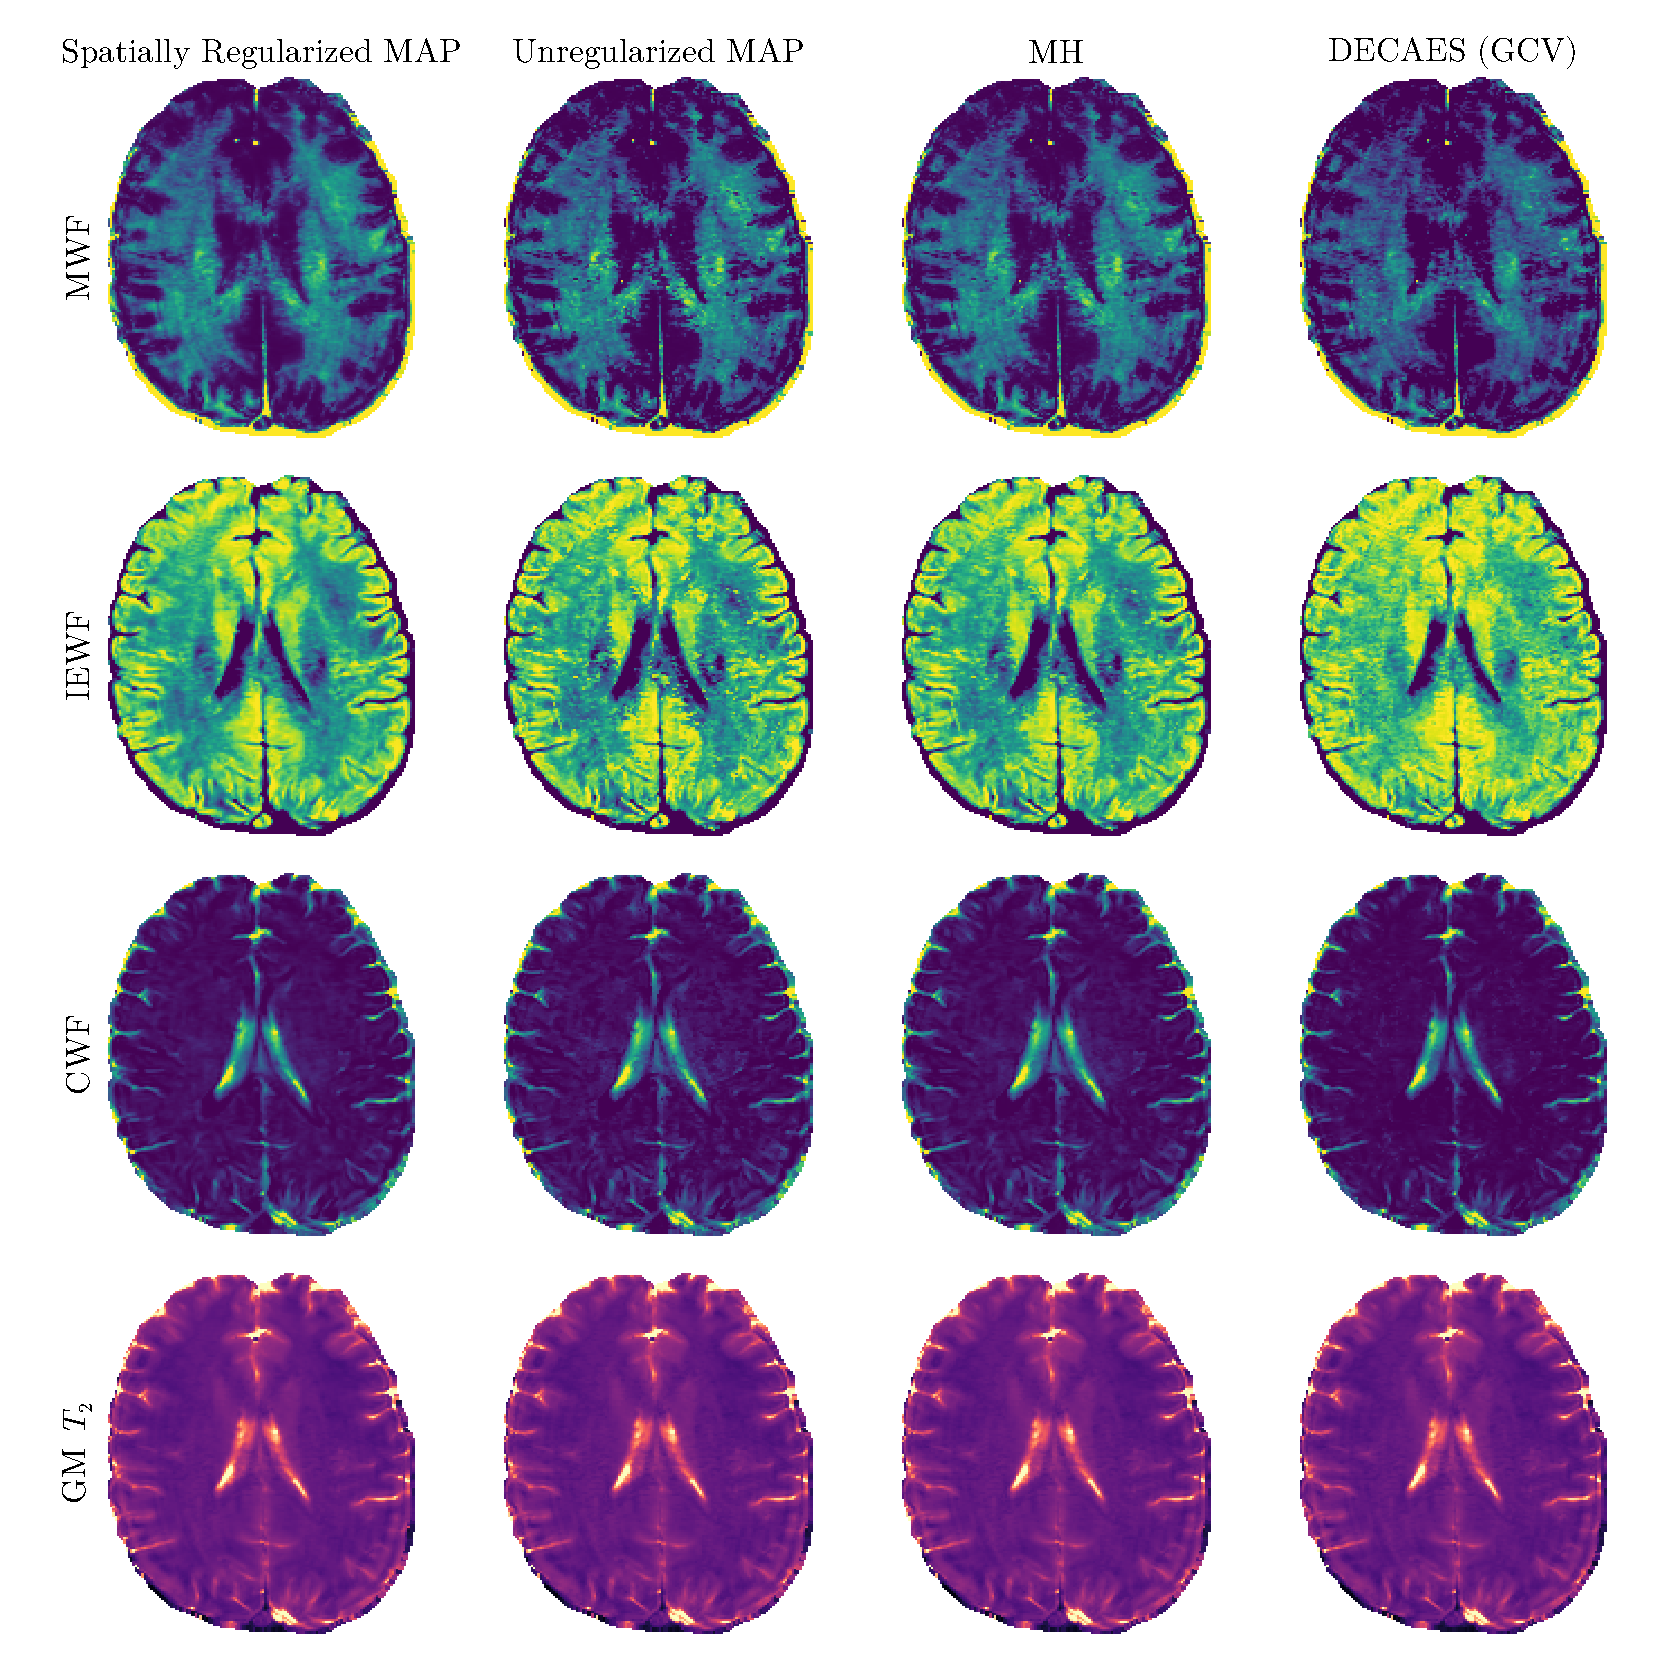
\includegraphics[width=\linewidth]{figures/spatial_map_observables.pdf}
    \caption{Spatially regularized two-step estimates. Biomarker maps derived from the spatially regularized \gls*{MAP} $T_2$ distribution are compared against the unregularized voxelwise \gls*{MAP} solution, the independent-proposal \gls*{MH} posterior mean, and \gls*{DECAES} with \gls*{GCV} regularization. The spatial prior smooths the estimates while preserving tissue boundaries.}
    \label{fig:spatial_map_observables}
\end{figure*}

Thus far we have considered only inference methods that are voxelwise-independent, with no voxel being influenced by its neighbours.
For virtually all inference problems in \gls*{MRI}, some degree of spatial regularity is expected \textit{a priori}, since the underlying tissue is organized into large, smoothly varying structures.
In myelin water imaging of the brain, $T_2$ spectra are expected to vary smoothly within the grey and white matter tissue compartments, since it is atypical for the underlying tissue to have sharp discontinuities.
This motivates the introduction of a spatial smoothing prior to couple the voxelwise estimates~\citep{kumar_using_2018,labadie_myelin_2014}.
We can impose this property \textit{after} training the voxelwise model components by modifying the learned prior over $T_2$ spectra such that continuity across voxels is encouraged.

The natural coordinates in which to impose smoothness are the \textit{whitened} \gls*{ILR} coordinates $\xi_i = \Lambda^{-1} \ILR{\bar{\distbn}_i; \beta_0} \in \mathbb{R}^{n_{T_2} - 1}$, where $i$ is a voxel index and $\Lambda$ is the learned low-pass window of~\cref{eqn:gaussian_window}.
These are the base coordinates of the low-pass prior~\eqref{eqn:low_pass_prior}, equal to the \gls*{DCT}-II coefficients of $\log \bar{\distbn}_i$ before multiplication by $\Lambda$.
Smoothing $\xi$ across voxels encourages spatial correlations in the corresponding $T_2$ distributions, with derived biomarkers smoothed implicitly.
We choose the simplest multivariate normal prior that imposes spatial correlations, a Gaussian Markov random field (\gls*{GMRF})~\citep{rue_gaussian_2005}.

Let $\mathcal{A}$ be the weighted adjacency matrix of the masked grid of voxels and let $D = \Diag{\vv{d}}$ be the diagonal matrix of voxel \textit{degrees};
that is, $\vv{d}_i = \sum_j \mathcal{A}_{ij}$ is the total weight of the edges incident to the $i^\text{th}$ voxel.
The corresponding symmetric normalized adjacency and graph Laplacian matrices are defined as
\begin{align}\label{eqn:apx:spatial_laplacian}
    W = D^{-1/2} \mathcal{A} D^{-1/2}, \quad L = \Id - W.
\end{align}
The standard-normal prior $p(\xi) = \mathcal{N}(\xi \mid \Zero, \Id)$ on $\xi$ has an identity precision matrix.
Here, we replace it with a block-diagonal \gls*{GMRF} prior with
\begin{align}\label{eqn:apx:spatial_precision}
    Q = \alpha \Id + \beta L = \alpha (\Id + \kappa L),
\end{align}
repeated $n_{T_2} - 1$ times on the diagonal;
$\alpha > 0$ controls the isotropic shrinkage, and $\beta \ge 0$ is a roughness penalty.
Because the learned prior over $\xi$ has unit marginal variance, we fix $\alpha = 1$ such that $Q = \Id + \kappa L$ depends only on the smoothing strength $\kappa \ge 0$.
Note that $W$ has eigenvalues contained in $[-1, 1]$, and assuming the brain mask is connected,\footnote{If the mask is not connected, there is one such eigenvector for each connected component. Given a partition of unity $\One = \sum_R \One_R$ over connected regions $R$, the corresponding eigenvectors are $\vv{d}^{1/2} \odot \One_R$.}
$\vv{d}^{1/2}$ is the unique eigenvector with unit eigenvalue, following from $\mathcal{A} \One = \vv{d}$.
Therefore $L$ is positive semidefinite with a one-dimensional null space and eigenvalues in $[0, 2]$, and $Q$ is positive definite for all $\kappa \ge 0$.

The global objective is a \gls*{MAP} optimization problem with respect to the joint base-coordinate measure of~\eqref{eqn:posterior_sampling_uspace}, in which the standard-normal prior on $\xi$ has been replaced by the \gls*{GMRF} prior:
\begin{align}\label{eqn:apx:spatial_energy}
    E(\vv{u})
    =
    \sum_{i = 1}^N -\log p(\vv{u}_i, \signal_i)
    + \frac{\kappa}{2} \sum_{j=1}^{n_{T_2}-1} \xi^{(j)}(\vv{u})^T L \xi^{(j)}(\vv{u}).
\end{align}
The first term is the usual voxelwise \gls*{MAP} objective in $\vv{u}$ coordinates, summing the independent negative log joint densities;
the second is the roughness penalty -- the difference between the spatial prior and the i.i.d.\ prior -- summed across coordinates, coupling neighbouring voxels.
There are now two tasks:
(1) to estimate the smoothing strength $\kappa$, and
(2) to minimize the energy objective~\eqref{eqn:apx:spatial_energy}.
The former is accomplished by an empirical Bayes approach, and the latter by a gradient-based optimization routine.

To estimate $\kappa$, we maximize an evidence lower bound on the marginal evidence $p(\signal \mid \kappa)$, similar to the flip-angle estimation in \cref{sec:apx:flip_angle_elbo}.
Because the block-diagonal prior factorizes over coordinates, it suffices to consider a single coordinate.
Let the trained amortized posterior $q(\xi \mid \signal)$ be the proposal distribution, where we drop the coordinate superscript on $\xi$ for brevity.
Then, the \gls*{ELBO} is given by the expected joint log density $\mathbb{E}_{q}[\log p(\signal, \xi \mid \kappa)]$ plus the entropy of $q$;
since the likelihood $p(\signal \mid \xi)$ and entropy $\mathbb{E}_{q}[-\log q(\xi \mid \signal)]$ are independent of $\kappa$, maximizing the \gls*{ELBO} over $\kappa$ reduces to maximizing the expected log prior under $q$:
\begin{align}\label{eqn:apx:spatial_mstep_obj}
    \mathcal{L}(\kappa)
    =
    \mathbb{E}_{q}\!\left[ \log p(\xi \mid \kappa) \right]
    =
    \frac{1}{2} \log\lvert Q \rvert - \frac{1}{2} \mathbb{E}_{q}\!\left[ \xi^T Q \xi \right] + \mathrm{const},
\end{align}
where we have substituted the Gaussian log-density $\log p(\xi \mid \kappa) = \tfrac{1}{2} \log\lvert Q \rvert - \tfrac{1}{2} \xi^T Q \xi + \mathrm{const}$.
By expanding the quadratic form $\xi^T Q \xi = \xi^T \xi + \kappa \xi^T L \xi$, we see that $\mathcal{L}$ depends on $q$ only via the sufficient statistics
\begin{align}\label{eqn:apx:spatial_stats}
    E_I & = \mathbb{E}_{q}\!\left[ \xi^T \xi \right],                         \\
    E_W & = \mathbb{E}_{q}\!\left[ \xi^T W \xi \right], \nonumber             \\
    E_L & = E_I - E_W = \mathbb{E}_{q}\!\left[ \xi^T L \xi \right], \nonumber
\end{align}
thus simplifying the \gls*{ELBO} objective and its derivative to
\begin{align}\label{eqn:apx:spatial_mstep}
    \mathcal{L}(\kappa)  & = \frac{1}{2} f(\kappa) - \frac{1}{2}( E_I + \kappa E_L ) + \mathrm{const}, \\
    \mathcal{L}'(\kappa) & = \frac{1}{2}\left( f'(\kappa) - E_L \right), \nonumber
\end{align}
where $f(\kappa) = \log\lvert \Id + \kappa L \rvert$ and $f'(\kappa) = \Tr{(\Id + \kappa L)^{-1} L} = \sum_i \frac{\lambda_i}{1 + \kappa \lambda_i}$, with $\lambda_i \in [0, 2]$ the eigenvalues of $L$.
Since $f'$ is strictly decreasing in $\kappa$ from $f'(0) = \Tr{L}$ to $f'(\infty) = 0$, a positive root of $f'(\kappa) = E_L$ exists and is unique whenever $0 < E_L < \Tr{L}$;
for $E_L \ge \Tr{L}$, the maximizer is the boundary value $\kappa = 0$, indicating no smoothing penalty.
Since $q$ factorizes over voxels and $L$ has unit diagonal, $E_L = \bar{\xi}^T L \bar{\xi} + \sum_i \mathrm{Var}_q(\xi_i)$ with $\bar{\xi} = \mathbb{E}_q[\xi]$.
The amortized posterior is trained under the i.i.d.\ prior, so in coordinates that a single voxel's data barely inform, $\mathrm{Var}_q(\xi_i)$ stays close to the prior variance and the variance term alone drives $E_L$ toward $\Tr{L}$ and $\kappa$ toward zero.
We therefore evaluate the statistics at the posterior mean, $E_I = \bar{\xi}^T \bar{\xi}$ and $E_L = \bar{\xi}^T L \bar{\xi}$, a plug-in empirical Bayes estimate computed without finite-sample bias from posterior samples by U-statistics.
Then $E_L = 0$ only if $\bar{\xi}$ is proportional to the null eigenvector $\vv{d}^{1/2}$, which would imply $\kappa \to \infty$.
We have two obvious choices to extend the single-coordinate analysis to the multi-coordinate case:
independent $\kappa_j$ can be fit to the respective coordinate statistics $E_I^{(j)}$ and $E_L^{(j)}$, or a single global $\kappa$ shared across coordinates can be fit to the average statistics $\bar{E}_I = \tfrac{1}{n_{T_2} - 1} \sum_j E_I^{(j)}$ and $\bar{E}_L = \tfrac{1}{n_{T_2} - 1} \sum_j E_L^{(j)}$.
We choose to use a shared global $\kappa$ for simplicity.

\begin{figure*}[th]
    \centering
    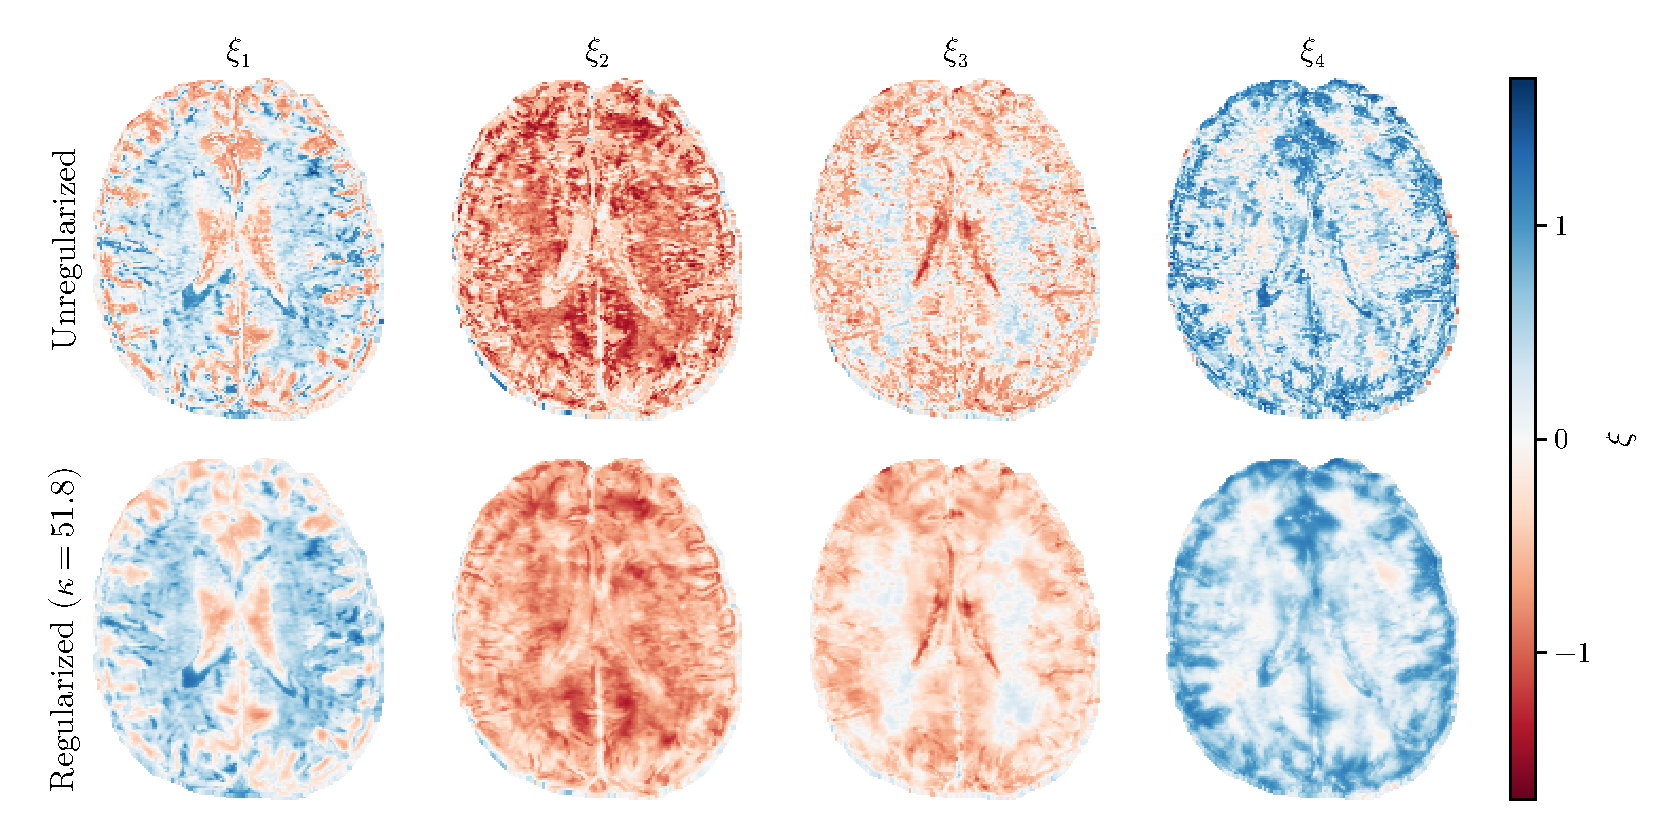
\includegraphics[width=\linewidth]{figures/spatial_map_ilr_fields.pdf}
    \caption{Effect of incorporating the spatial smoothing prior into the \gls*{MAP} estimate on the first four whitened \gls*{ILR} coordinates $\xi$.}
    \label{fig:spatial_map_ilr_fields}
\end{figure*}

After estimating $\kappa$, the spatially regularized solution $\vv{u}^*$ is found by minimizing~\cref{eqn:apx:spatial_energy} over $\vv{u}$, initialized at the pseudo-mode $\vv{u} = \Zero$.
The nuisance coordinates $\vv{u}_{\eta} = \Zero$ remain fixed at the conditional Laplace mode.
Optimization uses \textsc{PSGD} with a low-rank Newton-type preconditioner fitted to Hessian-vector products~\citep{li_preconditioned_2018,li_stochastic_2025}.
This results in smooth and spatially coherent images:
\cref{fig:spatial_map_observables} shows more spatially consistent biomarker maps than the unregularized \gls*{MAP} solution and the \gls*{MH} and \gls*{DECAES} baselines, and \cref{fig:spatial_map_ilr_fields} illustrates the corresponding spatial smoothing of the $\xi$ coordinates under the spatial prior.

\begin{figure*}[th]
    \centering
    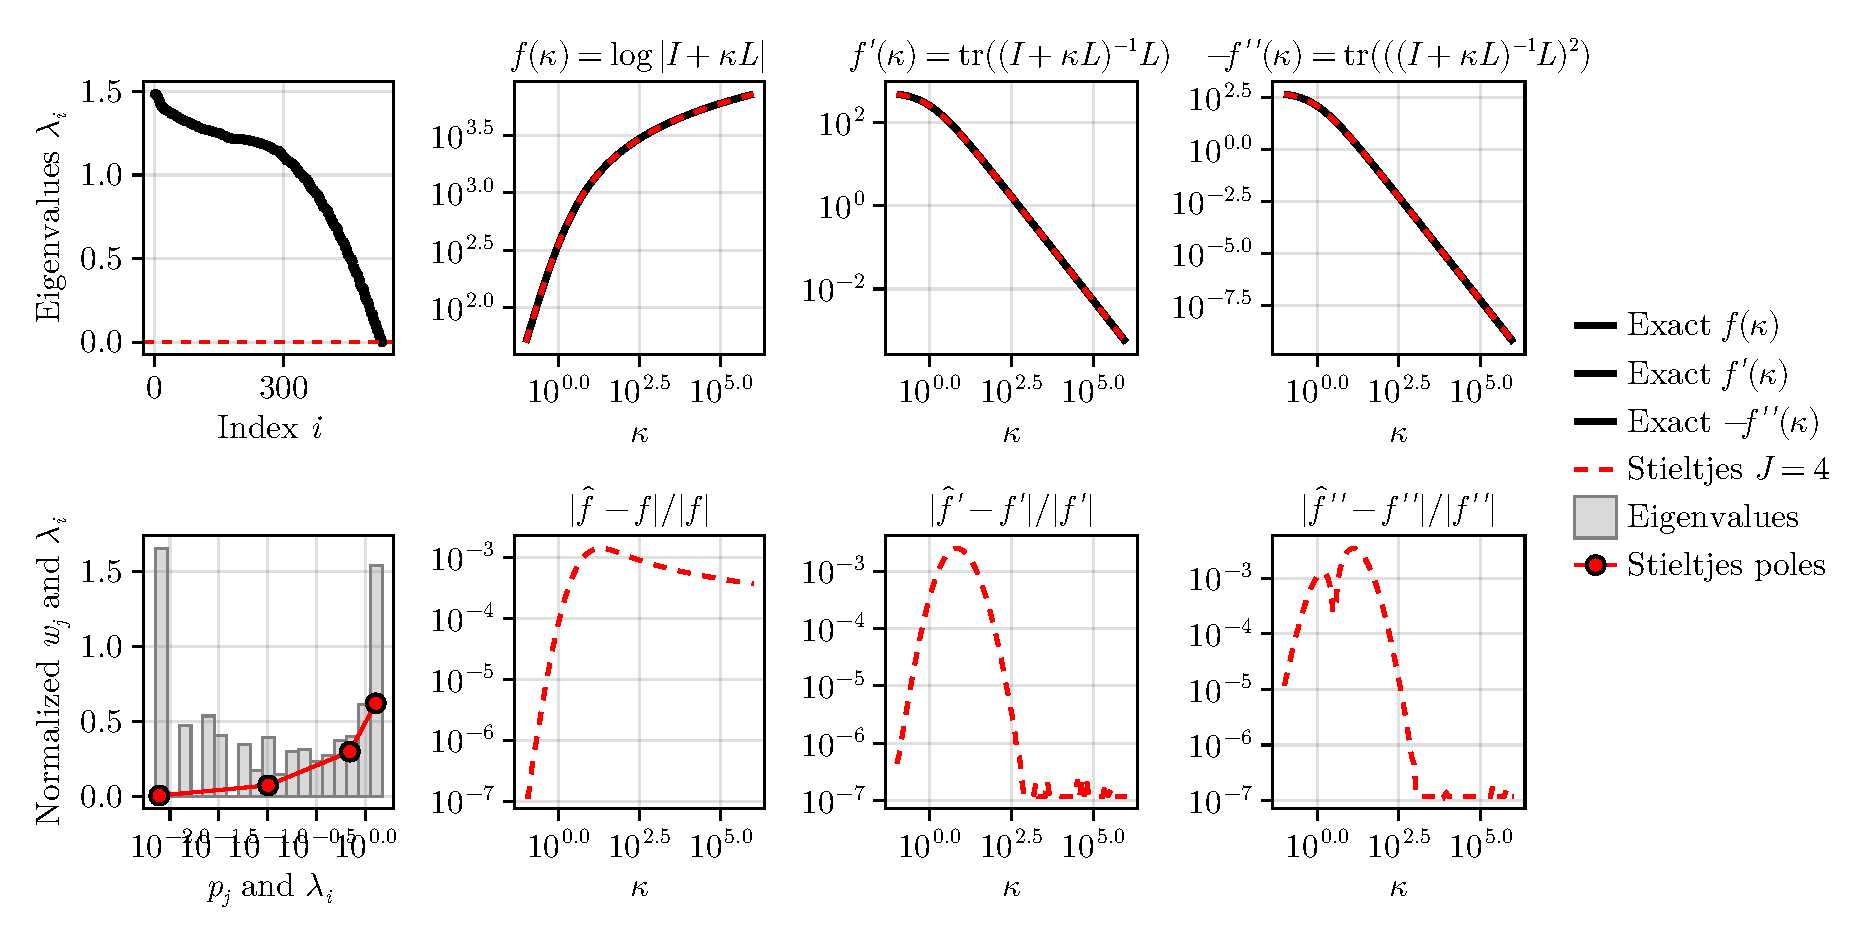
\includegraphics[width=\linewidth]{figures/spatial_stieltjes_validation.pdf}
    \caption{Comparison of the Stieltjes approximant ($J=4$ poles) against closed-form expressions for the operator $L$ on a central $23\times23$ crop of the selected slice. Top row: sorted eigenvalue spectrum of $L$, followed by exact and approximated values of $f(\kappa)$, $f'(\kappa)$, and $f''(\kappa)$. Bottom row: fitted poles and weights alongside the positive-eigenvalue histogram, followed by the relative approximation errors for $f(\kappa)$, $f'(\kappa)$, and $f''(\kappa)$.}
    \label{fig:spatial_stieltjes_validation}
\end{figure*}

\subsubsection{Efficient Log-Determinant Evaluation by Spectral Moment Matching}\label{subsubsec:apx:spatial_logdet}

Estimating the log-determinant $f(\kappa) = \log\lvert \Id + \kappa L \rvert$ and its derivative for a graph of $N \sim 10^6$ voxels is nontrivial, since full eigendecomposition of $L$ is impractically slow even if the graph is sparse.
The derivative is, however, a \textit{Stieltjes function}~\citep{stieltjes_recherches_1894} of the spectral measure of $L$,
\begin{align}\label{eqn:apx:spatial_stieltjes_exact}
    f(\kappa)  & = \log\lvert \Id + \kappa L \rvert = \sum_{i = 1}^N \log(1 + \kappa \lambda_i),                   \\
    f'(\kappa) & = \Tr{(\Id + \kappa L)^{-1} L} = \sum_{i = 1}^N \frac{\lambda_i}{1 + \kappa \lambda_i}, \nonumber
\end{align}
where $\lambda_i$ are the eigenvalues of $L$.
We approximate $f'$ by a $J$-pole rational function~\citep{golub_matrices_2009}
\begin{align}\label{eqn:apx:spatial_stieltjes_approx}
    f'(\kappa) \approx \sum_{j=1}^{J} \frac{w_j p_j}{1 + \kappa p_j}
\end{align}
whose poles $p_j > 0$ and weights $w_j > 0$ are chosen such that the approximant matches the asymptotic behaviour of $f'(\kappa)$ and its $J-1$ derivatives as $\kappa \to 0^+$ and $\kappa \to \infty$, respectively.
This requires estimating $\Tr{L^k} = \sum_i \lambda_i^k$ for $1 \le k \le J$ and $\Tr{(L^\dagger)^{k}} = \sum_{\lambda_i>0} \lambda_i^{-k}$ for $0 \le k \le J-1$, where $L^\dagger$ is the Moore--Penrose pseudo-inverse of $L$.
The log-determinant approximation is then given by integrating the rational approximant term by term, $f(\kappa) \approx \sum_j w_j \log(1 + \kappa p_j)$.
We will also evaluate the accuracy of the rational approximation to $f''(\kappa) = -\Tr{((\Id + \kappa L)^{-1}L)^2}$, given by similar term-by-term differentiation as $f''(\kappa) \approx -\sum_j w_j p_j^2/(1+\kappa p_j)^2$.
This moment-matching approach is equivalent to $J$-point Gaussian quadrature under the spectral measure of $L$, where the poles $p_j$ are quadrature nodes and $w_j$ are weights~\citep{golub_matrices_2009}.
The forward moments $\Tr{L^k}$ can be computed from $\Tr{W^k}$, which, for small $k$, can be computed reasonably fast from summing over all closed walks of length $k$ on the adjacency graph~\citep{cvetkovic_spectra_1980}.
The pseudo-inverse moments $\Tr{(L^\dagger)^{k}}$ are estimated stochastically using Hutchinson's trace estimator~\citep{hutchinson_stochastic_1989} after deflating away the known null space of $L$.
\Cref{fig:spatial_stieltjes_validation} compares the $J=4$-pole approximants with the closed-form expressions in~\cref{eqn:apx:spatial_stieltjes_exact}, computed using exact eigenvalues of $L$ for a two-dimensional grid.

\subsection{Inference at a Different \texorpdfstring{$T_2$}{T2} Resolution}\label{sec:apx:cross_resolution}

While the learned change of variables acts on a fixed bin count $n_{T_2}$, each simplex sample $\bar{\distbn}$ can be interpreted as a discretization of an underlying continuous $T_2$ density arising from a continuum of isochromats that each relax with their own $T_2$.
The same trained components can therefore be reused at a different bin count $n'_{T_2} \neq n_{T_2}$, holding the physical range $(T_2^{\min}, T_2^{\max})$ fixed.
This section compares two distinct ways to \textit{lift} $T_2$ inference to a higher resolution.
In the deterministic, or \textit{pseudo}, lift, the native posterior is sampled and each output distribution $\bar{\distbn}$ is then upsampled onto the target grid.
The \textit{product} lift instead samples the full $n'_{T_2}$-dimensional latent space, appending independent standard-normal high-frequency modes -- the directions the trained flow never modelled -- and evaluating the likelihood against the target-resolution basis $\epgbases_{n'}$.

Write $\ell = \log T_2$ and let $\Delta\ell = \log(T_2^{\max} / T_2^{\min}) / (n_{T_2} - 1)$, with $\Delta\ell'$ defined analogously at $n'_{T_2}$.
At any resolution, a simplex sample $\bar{\distbn}$ approximates the same continuous density via
\begin{align}\label{eqn:apx:cross_res_bin_mass}
    \bar{\distbn}_i \approx p(\ell_i) \Delta\ell, \quad p(\ell) \propto e^{g(\ell)},
\end{align}
where $g$ is a centred continuous logit field defined up to an additive constant.
Cross-resolution inference amounts to the claim that the same $g$ admits a faithful discretization on any grid spanning this physical range.
The softmax normalization in $\InvILR{\cdot; \beta_0}$~\eqref{eqn:inv_ilr_transform} supplies the bin-width factor in~\eqref{eqn:apx:cross_res_bin_mass}.
\Cref{sec:apx:simplex_distributions_asymptotics} shows that the corresponding \gls*{DCT} coefficients scale by $\sqrt{n'_{T_2} / n_{T_2}}$ between grids, while the bandwidth $F_c$ transfers unchanged as a physical log-$T_2$ frequency.

\subsubsection{Deterministic Lift by Interpolation}

The trained generator maps the latent base vector $\vv{u} \in \mathbb{R}^{n_{T_2} - 1}$, with $\vv{u} \sim \pi_{\vv{u}} = \mathcal{N}(\Zero, \Id_{n_{T_2} - 1})$, to a native-resolution distribution
\begin{align}\label{eqn:apx:cross_res_trained_gen}
    \varphi_{\bar{\distbn}}(\vv{u}; \signal) = \InvILR{\Lambda \varphi(\vv{u}; \signal); \beta_0},
\end{align}
where $\varphi(\cdot; \signal)$ is the trained Aitchison-space backbone and $\Lambda$ is the trained low-pass window of~\eqref{eqn:gaussian_window}.
The deterministic, or \textit{pseudo}, lift performs inference in this trained dimension and maps each posterior draw onto the target grid.
Let $L \in \mathbb{R}^{n'_{T_2} \times n_{T_2}}$ be a nonnegative column-stochastic matrix that redistributes native bin masses onto the target grid -- for instance the piecewise-linear interpolation matrix -- so that $\bar{\distbn}' = L\bar{\distbn}$ is a valid target-resolution distribution for any $\bar{\distbn} \in \ProbSimplex{n_{T_2} - 1}$.
Applying $L$ to a trained posterior draw then defines the deterministic lift
\begin{align}\label{eqn:apx:cross_res_deterministic_lift}
    \bar{\distbn}'(\vv{u}) = L \varphi_{\bar{\distbn}}(\vv{u}; \signal), \quad \vv{u} \sim q_{\vv{u}}(\vv{u} \mid \signal).
\end{align}
The trained encoder and the native sampler operate in dimension $n_{T_2}$ and cannot be applied to the target-resolution operator $\epgbases_{n'}$ directly.
We therefore condition both on the composite \textit{sketch basis} $B = \epgbases_{n'} L$, which compresses $\epgbases_{n'}$ back to $n_{T_2}$ columns through $L$.
Column-stochasticity gives the associativity $B\bar{\distbn} = \epgbases_{n'}(L\bar{\distbn}) = \epgbases_{n'}\bar{\distbn}'$, so fitting $\bar{\distbn}$ against $B$ is identical to fitting the lifted distribution $\bar{\distbn}'$ against the full target-resolution forward model.
The sampled $\bar{\distbn}$ is therefore not itself a $T_2$ distribution; it is a trained-dimension coordinate, likely under the trained prior, whose interpretable target-resolution image is $\bar{\distbn}' = L\bar{\distbn}$.
Sampling remains $n_{T_2}$-dimensional, but replacing $A$ by $B$ changes both the likelihood and the encoder input, so the importance ratio need not be preserved.
In the experiments below, the effective sample size decreases only slightly with the pseudo-lift, but note also that the lift merely interpolates the trained representation, and thus cannot recover target-resolution structure outside the column span of $L$.

\subsubsection{Lifted Flow Construction}

The product lift splices the trained backbone $\varphi$ of~\eqref{eqn:apx:cross_res_trained_gen} with an identity flow on the added coordinates.
It operates on the padded base vector $\vv{u}' = (\vv{u}, \vv{v}) \in \mathbb{R}^{n'_{T_2} - 1}$ with $\vv{v} \sim \mathcal{N}(\Zero, \Id_{n'_{T_2} - n_{T_2}})$ and is given explicitly by
\begin{align}\label{eqn:apx:cross_res_lifted_gen}
    \varphi_{\bar{\distbn}'}(\vv{u}'; \signal) = \InvILR{\Lambda' (\varphi \oplus \Id)(\vv{u}'; \signal); \beta_0},
\end{align}
where $\varphi \oplus \Id$ passes the first $n_{T_2} - 1$ coordinates through the trained backbone $\varphi$ and the remaining $n'_{T_2} - n_{T_2}$ coordinates through the identity, $\InvILR{\cdot; \beta_0}$ uses the target-resolution basis $\Psi'$ from~\eqref{eqn:apx:cross_res_psi_def}, and $\Lambda'$ is the lifted window with diagonal entries
\begin{align}\label{eqn:apx:cross_res_lifted_window}
    \lambda'_i = \sqrt{\frac{n'_{T_2}}{n_{T_2}}} \lambda_i^{+}(f'_i), \quad f'_i = \frac{i}{n_{T_2}},
\end{align}
where $\lambda_i^{+}$ is the noise-floored window of~\eqref{eqn:gaussian_window}.
The prefactor implements the coefficient scaling in~\eqref{eqn:apx:cross_res_dct_scaling}.
The normalized frequency $f'_i$ is divided by the trained bin count rather than the target bin count, preserving the physical bandwidth $F_c$ from~\eqref{eqn:gaussian_window}.

\subsubsection{Lifted Prior, Likelihood, and Importance Ratio}

The lifted prior on $\bar{\distbn}'$ mirrors~\eqref{eqn:apx:cross_res_lifted_gen} with $\varphi$ replaced by the identity,
\begin{align}\label{eqn:apx:cross_res_lifted_prior}
    \bar{\distbn}' = \InvILR{\Lambda' \vv{u}'; \beta_0}, \quad \vv{u}' \sim \mathcal{N}(\Zero, \Id_{n'_{T_2} - 1}),
\end{align}
yielding a low-pass windowed distribution on $\ProbSimplex{n'_{T_2} - 1}$.
The quantized Rician likelihood~\eqref{eqn:signal_likelihood} is evaluated against the lifted $\bar{\distbn}'$ and the target-resolution \gls*{EPG} basis $\epgbases_{n'}$, built from the same physical acquisition parameters as $\epgbases_{n}$.
Laplace's approximation~\eqref{eqn:laplace_approximation} for the nuisance parameters $\log s$ and $\log \sigma$ is likewise reconditioned on $\bar{\distbn}'$ and $\epgbases_{n'}$, so that they are estimated against the same forward operator the likelihood uses.
The encoder, by contrast, still requires the trained dimension and is conditioned on the same sketch basis $B = \epgbases_{n'} L$ as the deterministic lift.

Since the trained backbone $\varphi$ acts only on the first $n_{T_2} - 1$ base coordinates and $\vv{v}$ passes through the identity in \textit{both} the lifted generator~\eqref{eqn:apx:cross_res_lifted_gen} and the lifted prior~\eqref{eqn:apx:cross_res_lifted_prior}, the base-coordinate densities factor identically as
\begin{align}\label{eqn:apx:cross_res_density_factorization}
    \pi_{\vv{u}'}(\vv{u}, \vv{v})            & = \pi_{\vv{u}}(\vv{u}) \cdot \mathcal{N}(\vv{v} \mid \Zero, \Id),            \\
    q_{\vv{u}'}(\vv{u}, \vv{v} \mid \signal) & = q_{\vv{u}}(\vv{u} \mid \signal) \cdot \mathcal{N}(\vv{v} \mid \Zero, \Id).
\end{align}
The forward Jacobians of the lifted flow therefore cancel in the independent-Metropolis importance ratio, as do the $\mathcal{N}(\vv{v} \mid \Zero, \Id)$ base-density factors, leaving the trained-resolution ratio multiplied only by the likelihood contribution in $\vv{v}$.
If the likelihood were independent of $\vv{v}$, the lifted importance ratio would reduce exactly to the trained one and Monte Carlo efficiency would be independent of $n'_{T_2} - n_{T_2}$;
in practice, $\vv{v}$ enters the likelihood through $\InvILR{\cdot; \beta_0}$ and $\epgbases_{n'}$, so a residual high-mode mismatch produces finite importance-ratio variance.
The experiments below compare the deterministic lift, the full product proposal, and a recentred product proposal that first shifts the lifted latent coordinates to their posterior mode.

\subsubsection{Posterior Mode Recentring}

The product lift in~\eqref{eqn:apx:cross_res_lifted_gen} uses the prior as the proposal for the added high modes.
If the posterior mode in the lifted coordinates is displaced from $\vv{u}' = \Zero$, then independent proposals waste samples near the wrong centre even when the local approximate posterior shape is reasonable.
This motivates a shifted product proposal.
Let $\vv{u}^*$ minimize the lifted negative log posterior using the same free energy as the sampler, with the encoder conditioned on $\epgbases_{n'} L$ and the likelihood evaluated using $\epgbases_{n'}$.
The shifted generator is
\begin{align}\label{eqn:apx:cross_res_map_shift}
    \varphi^{\mathrm{MAP}}_{\bar{\distbn}'}(\vv{u}'; \signal) = \varphi_{\bar{\distbn}'}(\vv{u}' + \vv{u}^*; \signal).
\end{align}
This shift has unit Jacobian and therefore changes only the proposal centre.

\subsubsection{Experiments}

\begin{table*}[htbp]
    \centering
    \small
    \resizebox{\linewidth}{!}{\begin{tabular}{ccccccccc}
  \toprule
  \textbf{$\mathrm{Method}$} & \textbf{$n_{T_2}$} & \textbf{$\alpha_{\mathrm{MH}}$} & \textbf{$\alpha_{\mathrm{RWM}}$} & \textbf{$\alpha_{\mathrm{MALA}}$} & \textbf{$\mathrm{ESS}_{\mathrm{IS}}/S$} & \textbf{$\tau_{\mathrm{MH}}$} & \textbf{$\tau_{\mathrm{RWM}}$} & \textbf{$\tau_{\mathrm{MALA}}$} \\
  \midrule
  Native                     & 41                 & $0.793^{0.81}_{0.77}$           & $0.234^{0.24}_{0.23}$            & $0.548^{0.56}_{0.54}$             & $0.847^{0.87}_{0.8}$                    & $1.68^{2.0}_{1.5}$            & $58.2^{80.0}_{43.0}$           & $6.32^{7.7}_{5.3}$              \\
  Native + MAP               & 41                 & $0.771^{0.8}_{0.74}$            & $0.234^{0.24}_{0.23}$            & $0.55^{0.56}_{0.54}$              & $0.82^{0.85}_{0.76}$                    & $1.72^{2.1}_{1.5}$            & $57.4^{80.0}_{41.0}$           & $6.34^{7.5}_{5.2}$              \\
  Product                    & 81                 & $0.384^{0.52}_{0.26}$           & $0.223^{0.23}_{0.21}$            & $0.372^{0.46}_{0.28}$             & $0.181^{0.35}_{0.075}$                  & $6.42^{13.0}_{3.8}$           & $82.6^{110.0}_{60.0}$          & $13.1^{20.0}_{9.6}$             \\
  Product + MAP              & 81                 & $0.511^{0.6}_{0.41}$            & $0.223^{0.23}_{0.21}$            & $0.374^{0.46}_{0.28}$             & $0.303^{0.48}_{0.14}$                   & $4.03^{6.7}_{2.8}$            & $82.2^{110.0}_{57.0}$          & $13.5^{21.0}_{9.4}$             \\
  Pseudo-lift                & 81                 & $0.756^{0.79}_{0.7}$            & $0.234^{0.24}_{0.23}$            & $0.549^{0.56}_{0.54}$             & $0.798^{0.85}_{0.71}$                   & $1.81^{2.3}_{1.6}$            & $59.2^{79.0}_{42.0}$           & $6.32^{7.6}_{5.2}$              \\
  Pseudo-lift + MAP          & 81                 & $0.766^{0.79}_{0.73}$           & $0.234^{0.24}_{0.23}$            & $0.548^{0.56}_{0.53}$             & $0.809^{0.85}_{0.74}$                   & $1.76^{2.1}_{1.5}$            & $56.2^{79.0}_{40.0}$           & $6.23^{7.6}_{5.2}$              \\
  Product                    & 121                & $0.329^{0.47}_{0.2}$            & $0.225^{0.23}_{0.21}$            & $0.394^{0.48}_{0.31}$             & $0.133^{0.29}_{0.051}$                  & $7.95^{17.0}_{4.5}$           & $89.4^{120.0}_{62.0}$          & $14.8^{22.0}_{11.0}$            \\
  Product + MAP              & 121                & $0.506^{0.6}_{0.4}$             & $0.226^{0.23}_{0.22}$            & $0.397^{0.48}_{0.31}$             & $0.307^{0.48}_{0.16}$                   & $4.18^{7.4}_{2.8}$            & $93.0^{120.0}_{67.0}$          & $14.4^{21.0}_{10.0}$            \\
  Pseudo-lift                & 121                & $0.746^{0.78}_{0.68}$           & $0.234^{0.24}_{0.23}$            & $0.548^{0.56}_{0.53}$             & $0.786^{0.84}_{0.69}$                   & $1.89^{2.5}_{1.6}$            & $57.8^{82.0}_{42.0}$           & $6.41^{7.7}_{5.3}$              \\
  Pseudo-lift + MAP          & 121                & $0.762^{0.79}_{0.72}$           & $0.235^{0.24}_{0.23}$            & $0.548^{0.56}_{0.53}$             & $0.804^{0.84}_{0.73}$                   & $1.8^{2.2}_{1.6}$             & $56.3^{79.0}_{43.0}$           & $6.36^{7.7}_{5.3}$              \\
  \bottomrule
\end{tabular}
}
    \caption{Cross-resolution sampling diagnostics. Entries report median values with interquartile bounds across voxels. The native row is the trained-resolution reference; pseudo-lift denotes deterministic interpolation onto the target grid by~\eqref{eqn:apx:cross_res_deterministic_lift}; product denotes full $n'_{T_2}$-dimensional sampling; and \gls*{MAP} denotes recentring by~\eqref{eqn:apx:cross_res_map_shift}.}
    \label{tab:apx:cross_resolution_diagnostics}
\end{table*}

\begin{figure*}[htbp]
    \centering
    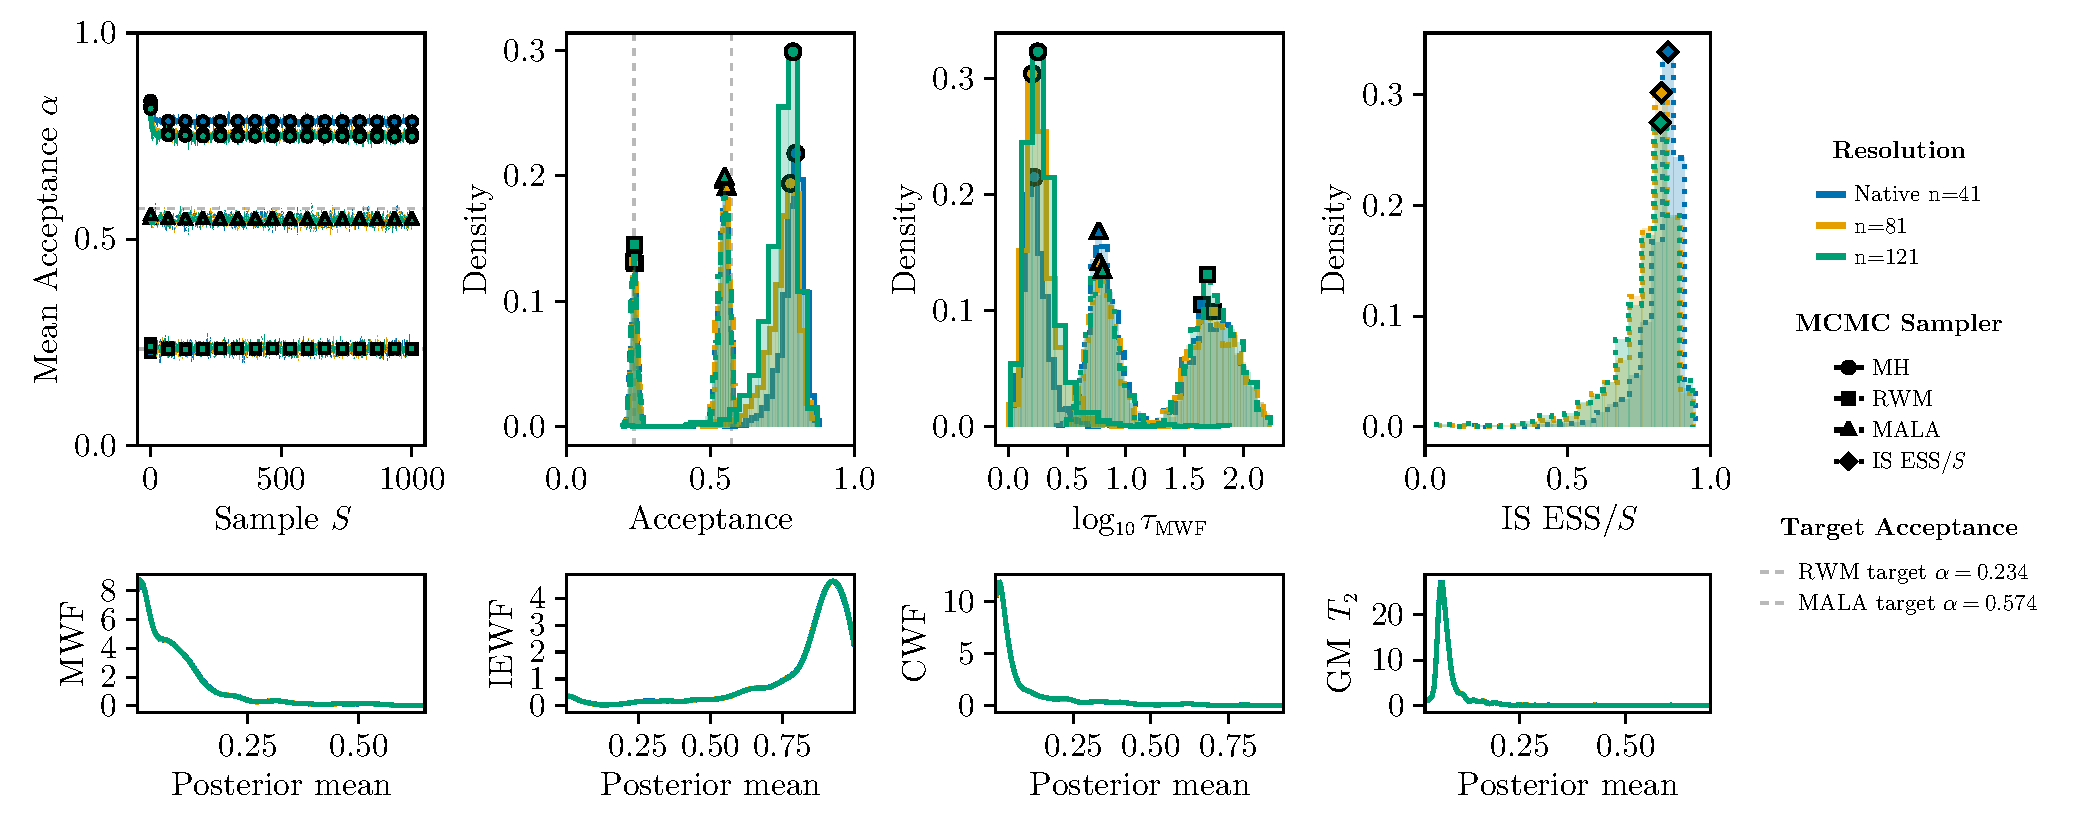
\includegraphics[width=\linewidth]{figures/cross_resolution_cohort_diagnostics.pdf}
    \caption{Cohort-level cross-resolution diagnostics for the pseudo-lift with \gls*{MAP} recentring. Acceptance trajectories, per-voxel acceptance distributions, \gls*{MWF} autocorrelation times, importance-sampling $\mathrm{ESS}/S$, and posterior-mean biomarker distributions are shown across target resolutions.}
    \label{fig:apx:cross_resolution_cohort}
\end{figure*}

\begin{figure*}[htbp]
    \centering
    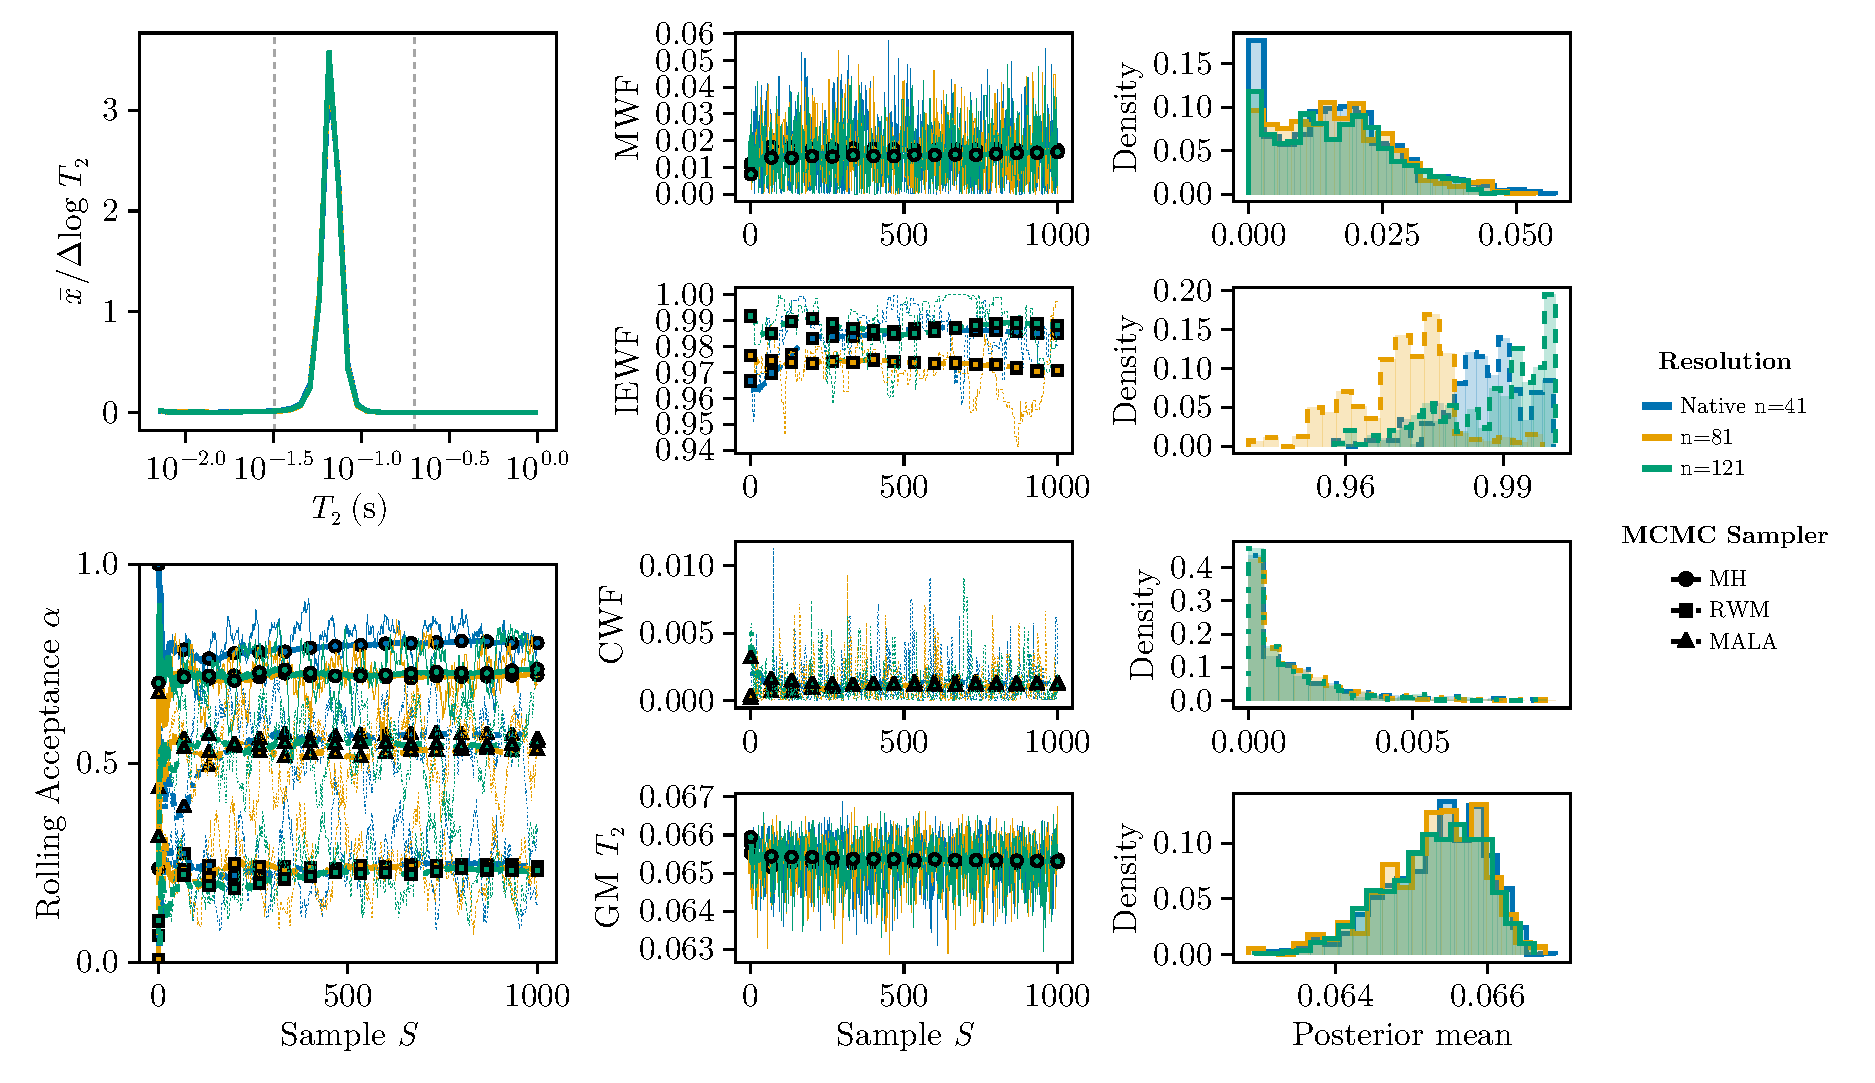
\includegraphics[width=\linewidth]{figures/cross_resolution_voxel_diagnostics.pdf}
    \caption{Voxel-level cross-resolution diagnostics for the pseudo-lift with \gls*{MAP} recentring.
    The top-left panel compares posterior $T_2$ densities, the bottom-left panel shows rolling independent-\gls*{MH} acceptance, and the remaining panels show biomarker traces and posterior biomarker distributions for one representative voxel.}
    \label{fig:apx:cross_resolution_voxel}
\end{figure*}

To assess cross-resolution inference, we compare the pseudo-lift~\eqref{eqn:apx:cross_res_deterministic_lift}, the product lift~\eqref{eqn:apx:cross_res_lifted_gen}, and the \gls*{MAP}-shifted product lift~\eqref{eqn:apx:cross_res_map_shift} at target resolutions $n'_{T_2} \in \{41, 81, 121\}$, holding $n_{T_2}$ fixed at the trained resolution.
The pseudo-lift samples the trained latent dimension against $\epgbases_{n'} L$ and then interpolates each posterior draw to the target grid.
The product methods sample the full lifted latent dimension against $\epgbases_{n'}$.

On the same ID test cohort, we ran independent \gls*{MH}, \gls*{RWM}, and \gls*{MALA}, using the step sizes of \cref{subsubsec:inference_details}, and importance sampling with the corresponding independent proposals.
\Cref{tab:apx:cross_resolution_diagnostics,fig:apx:cross_resolution_cohort,fig:apx:cross_resolution_voxel} report acceptance, autocorrelation, effective sample size, and biomarker diagnostics.

The pseudo-lift changed little with resolution, since it interpolates the native posterior without sampling added modes.
The unshifted product lift degraded as $n'_{T_2}$ increased;
\gls*{MAP} recentring recovered part of the degradation.

\section{Extended Phase Graph Algorithm}\label{sec:apx:epg_basis}

The extended phase graph (\gls*{EPG}) basis matrix $\epgbases \in \mathbb{R}_+^{n_{\TE} \times n_{T_2}}$ is constructed using the \gls*{EPG} algorithm, which accounts for $T_1$ and $T_2$ relaxation, stimulated echoes, and $B_1$-inhomogeneity~\citep{hennig_multiecho_1988,prasloski_applications_2012}.
Each column of $\epgbases$ is a vector containing the magnitudes of $n_{\TE}$ spin echoes, forming a simulated multi-spin echo (\gls*{MSE}) signal.
This signal is generated by evolving an initial magnetization state for $n_{\TE}$ periods of uniform echo spacing $\TE$.
The longitudinal relaxation time $T_1$ is the same for all columns, while the transverse relaxation time $T_{2,j}$ varies logarithmically from $T_2^{\min}$ (first column) to $T_2^{\max}$ (last column).
The $(i,j)^{\text{th}}$ entry of $\epgbases$ is given by
\begin{align}\label{eqn:epg_basis_definition}
    \epgbases_{i,j} = \lvert (\mathbf{M}^{i,j})_1^+ \rvert,
\end{align}
where $\mathbf{M}^{i,j} \in \mathbb{C}^{3 n_{\TE}}$ is a \textit{magnetization phase state vector} (\gls*{MPSV}) of $n_{\TE}$ spin population phase states.
Each phase state $(\mathbf{M}^{i,j})_{k}$ is represented by a triplet $((\mathbf{M}^{i,j})_k^+, (\mathbf{M}^{i,j})_k^-, (\mathbf{M}^{i,j})_k^z)$ of Fourier coefficients, where $(\mathbf{M}^{i,j})_k^+$ and $(\mathbf{M}^{i,j})_k^-$ are the positive- and negative-order coefficients of the simulated complex transverse magnetization $M_{xy} = M_x + i M_y$, and $(\mathbf{M}^{i,j})_k^z$ is the corresponding coefficient of the simulated real longitudinal magnetization $M_z$.

The \gls*{MPSV} $\mathbf{M}^{i,j}$ is computed via the propagation equations
\begin{align}\label{eqn:mpsv_definition}
    \begin{cases}
        \quad \mathbf{M}^{i,j} & = \vv{E}_{j} \vv{S} \vv{R}_{j} \vv{E}_{j} \mathbf{M}^{i-1,j} \quad (1 \leq i \leq n_{\TE}), \\
        (\mathbf{M}^{0,j})_{1} & = (\sin\alpha_{\text{ex}}, 0, 0),                                                           \\
        (\mathbf{M}^{0,j})_{k} & = (0, 0, 0) \quad (2 \leq k \leq n_{\TE})
    \end{cases}
\end{align}
where $\alpha_{\text{ex}}$ is the excitation pulse flip angle.
The relaxation, rotation, and transition matrices $\vv{E}_{j}$, $\vv{R}_{j}$, and $\vv{S}$ are defined by their actions on an \gls*{MPSV} $\mathbf{M}$ as follows:
\begin{align}\label{eqn:epg_basis_components}
    (\vv{E}_{j} \mathbf{M})_{k} & =
    \begin{bmatrix}
        E_{2,j} & 0       & 0     \\
        0       & E_{2,j} & 0     \\
        0       & 0       & E_{1}
    \end{bmatrix}
    (\mathbf{M})_{k},               \\
    (\vv{R}_{j} \mathbf{M})_{k} & =
    \begin{bmatrix*}[r]
        \cos^2(\alpha_{j}/2)           & \sin^2(\alpha_{j}/2)          & -i \sin(\alpha_{j}) \\
        \sin^2(\alpha_{j}/2)           & \cos^2(\alpha_{j}/2)          &  i \sin(\alpha_{j}) \\
        -\tfrac{i}{2} \sin(\alpha_{j}) & \tfrac{i}{2} \sin(\alpha_{j}) &    \cos(\alpha_{j})
    \end{bmatrix*}
    (\mathbf{M})_{k},               \\
    \vv{S} \mathbf{M}           & :
    \begin{cases}
        (\vv{S} \mathbf{M})_1^+           = (\mathbf{M})_1^-,                                       \\
        (\vv{S} \mathbf{M})_k^+           = (\mathbf{M})_{k-1}^+ \quad (2 \leq k \leq n_{\TE}),     \\
        (\vv{S} \mathbf{M})_k^-           = (\mathbf{M})_{k+1}^- \quad (1 \leq k \leq n_{\TE} - 1), \\
        (\vv{S} \mathbf{M})_{n_{\TE}}^-   = 0,                                                      \\
        (\vv{S} \mathbf{M})_k^z           = (\mathbf{M})_k^z.
    \end{cases}
\end{align}
Here, $(\mathbf{M}^{i,j})_k^+$ denotes the transverse component of the $k^{\text{th}}$ triplet of $\mathbf{M}^{i,j}$, and similarly $(\mathbf{M}^{i,j})_k^-$ and $(\mathbf{M}^{i,j})_k^z$ denote the anti-transverse and longitudinal components, respectively;
$E_{2,j} = \exp(-\frac{\TE/2}{T_{2,j}})$ and $E_{1} = \exp(-\frac{\TE/2}{T_{1}})$ are attenuation factors;
$\alpha_{\text{ex}} = \bar{\alpha} \frac{\pi}{2}$ and $\alpha_j \equiv \bar{\alpha} \pi$ are excitation and refocusing flip angles;
and $\bar{\alpha}(x, y, z) \in [0, 1]$ is a spatially varying map of $B_1$-inhomogeneity correction factors.
This $B_1$ map can be measured separately or estimated per voxel~\citep{prasloski_applications_2012,doucette_decaes_2020}.
For convenience we refer to $\alpha = \bar{\alpha} \pi$ as \textit{the} flip angle of a voxel, noting that $\alpha$ determines the excitation flip angle $\alpha_{\text{ex}} = \frac{\alpha}{2}$.

The \gls*{EPG} basis matrix $\epgbases$ is constructed efficiently using the \gls*{DECAES} open-source software package~\citep{doucette_decaes_2020}.

\section{Quantized Rician Noise Model}\label{sec:apx:rician_noise}

Magnitude \gls*{MRI} data is more accurately modelled with Rician rather than Gaussian noise~\citep{rice_mathematical_1944, rice_mathematical_1945, gudbjartsson_rician_1995}.
Given a true signal $\nu$ and noise level $\sigma$, the Rician probability density function (\gls*{PDF}) for the measured signal magnitude $x$ is:
\begin{align}\label{eqn:rician_pdf}
    p_{\Rice}(x \mid \nu, \sigma) = \frac{x}{\sigma^2} \exp\left(-\frac{x^2 + \nu^2}{2\sigma^2}\right) I_0\left(\frac{x\nu}{\sigma^2}\right),
\end{align}
where $I_0$ is the modified Bessel function of the first kind with order zero.

When the measurement $x$ is quantized to a resolution of $\delta$, the probability of observing $x$ given $\nu$ and $\sigma$ is the integral of $p_{\Rice}$ over the bin $[x, x + \delta)$:
\begin{align}\label{eqn:qrician_pdf}
    p_{\QRice}(x \mid \nu, \sigma, \delta) = \int_{0}^{\delta} p_{\Rice}(x + \epsilon \mid \nu, \sigma) \, d\epsilon.
\end{align}
We approximate $p_{\QRice}$ using Gauss--Legendre quadrature:
\begin{align}\label{eqn:qrician_quadrature}
    p_{\QRice}(x \mid \nu, \sigma, \delta) & \approx \frac{\delta}{2} \sum_{k=1}^{N} w_k p_{\Rice}\left(x_k \mid \nu, \sigma \right), \\
    x_k                                    & = x + \frac{\delta}{2}(1 + \xi_k), \nonumber
\end{align}
where $\xi_k \in (-1, 1)$ and $w_k > 0$ are the $N$ Gauss--Legendre nodes and weights.
We choose this method because $p_{\Rice}$ is analytic, and Gauss--Legendre quadrature is nearly optimal among quadrature rules for analytic functions~\citep{kowalski_is_1985,chawla_error_1968}.
The implementation uses $N = 8$ nodes and weights generated at compile time for likelihood evaluation and the final nuisance Hessian. Its automatic derivatives use the same quadrature rule.

Note that the accuracy of this non-adaptive quadrature depends on the integrand and the integration interval.
Pathological cases, such as $\delta \gg \sigma$ (a sharply peaked distribution relative to the integration domain) or $x \gg \nu$ (integration in the tail where $p_{\Rice}$ decays rapidly), can lead to errors.
While adaptive methods could address these issues, they introduce additional complexity and computational overhead.
In our posterior sampling application, the variational training optimizes for $\nu$ and $\sigma$ that are likely given $x$, encouraging $[x, x + \delta)$ to contain the Rician \gls*{PDF}'s mode.
We also expect $\sigma \gtrsim \delta$, since $\sigma$ is estimated from the data, and noise levels smaller than $\delta$ cannot be resolved due to quantization.
Thus, we integrate over small intervals near the mode, where $p_{\Rice}$ is slowly varying and well-suited for quadrature.

Our implementation of the Rician and quantized Rician probability density functions, including numerical integration and derivative calculations for automatic differentiation, is open-sourced at \url{https://github.com/jondeuce/FastRicianLikelihoods.jl}.
This implementation uses numerically stable expressions for the Rician log-density and its derivatives, including the explicit derivatives needed to compute Laplace's approximation in \cref{subsubsec:laplace_approximation}.

\section{Gaussian Initialization for Laplace's Approximation}\label{sec:apx:gaussian_approximation}

As described in \cref{subsubsec:laplace_approximation}, we use Newton's method to compute the mean $\mu_{\eta}$ for Laplace's approximation.
To obtain a suitable initial guess for this method, we approximate the posterior mode by substituting a Gaussian likelihood for the quantized Rician likelihood and solving for the mode of the resulting posterior.
We assume that $\bar{\distbn}$ is given and fixed (see Equation~\eqref{eqn:posterior_factorization}).

We approximate the quantized Rician likelihood model with a Gaussian likelihood model for the mean dequantized signal $\bar{\signal} = \signal + \delta / 2$, where $\delta$ denotes the quantization bin width.
This approximation is motivated by considering the simplest case where the quadrature in~\eqref{eqn:qrician_quadrature} is computed with only $N=1$ node.
In this case, the quantized Rician model is exactly equivalent to a Rician model evaluated at the mean dequantized signal $\bar{\signal}$.
For sufficiently large $\nu/\sigma$, this Rician model is itself well-approximated by a Gaussian likelihood.
Thus, to compute the initial guess, we minimize the negative log-joint posterior
\begin{align}
    -\log p(\eta, \bar{\signal} \mid \bar{\distbn}) & = -\log p(\bar{\signal} \mid \bar{\distbn}, \eta) - \log p(\eta \mid \bar{\distbn}) \label{eqn:gauss_approx_neg_log_joint}                \\
    \text{where} \quad
    -\log p(\bar{\signal} \mid \bar{\distbn}, \eta) & = \frac{n_{\TE}}{2} \log(2\pi\sigma^2) + \frac{\lVert \bar{\signal} - s\bar{\nu} \rVert^2}{2\sigma^2} \label{eqn:gauss_approx_likelihood}
\end{align}
is the Gaussian likelihood, $\bar{\nu} = \epgbases \bar{\distbn}$, and the prior $p(\eta \mid \bar{\distbn}) \equiv p(\eta)$ on the nuisance parameters $\eta = (\log s, \log \sigma)$ is taken to be independent of $\bar{\distbn}$.

We begin by computing the maximum likelihood estimate (\gls*{MLE}), i.e., the mode of the likelihood~\eqref{eqn:gauss_approx_likelihood}.
Setting the gradient of~\eqref{eqn:gauss_approx_likelihood} with respect to $\eta$ to zero yields:
\begin{align*}
    \vv{0} = \nabla_{\eta} \left[ -\log p(\bar{\signal} \mid \bar{\distbn}, \eta) \right] =
    \begin{pmatrix}
        -\frac{s}{\sigma^2} \bar{\nu} \cdot (\bar{\signal} - s \bar{\nu}) \\
        n_{\TE} - \frac{1}{\sigma^2} \lVert \bar{\signal} - s\bar{\nu} \rVert_2^2
    \end{pmatrix}.
\end{align*}
Solving for $s$ and $\sigma^2$ gives the maximum likelihood estimators:
\begin{align}\label{eqn:gauss_approx_mle}
    s_{\text{MLE}} = \frac{\bar{\nu} \cdot \bar{\signal}}{\lVert \bar{\nu} \rVert^2}
    \quad
    \sigma_{\text{MLE}}^2 = \frac{\lVert \bar{\signal} - s_{\text{MLE}}\bar{\nu} \rVert^2}{n_{\TE}}.
\end{align}
Equivalently, $s_{\text{MLE}}$ minimizes $\lVert \bar{\signal} - s\bar{\nu} \rVert^2$, and $\sigma_{\text{MLE}}^2$ is the mean square of the residuals $r = \bar{\signal} - s_{\text{MLE}}\bar{\nu}$.
We will also need the Hessian of~\eqref{eqn:gauss_approx_likelihood} at the \gls*{MLE}:
\begin{align*}
    H(\eta)                    & = \nabla_{\eta}^2 \left[ -\log p(\bar{\signal} \mid \bar{\distbn}, \eta) \right] \\
                               & =
    \begin{bmatrix}
        -\frac{s}{\sigma^2} \bar{\nu} \cdot (\bar{\signal} - 2s \bar{\nu}) & \frac{2s}{\sigma^2} \bar{\nu} \cdot (\bar{\signal} - s \bar{\nu}) \\
        \frac{2s}{\sigma^2} \bar{\nu} \cdot (\bar{\signal} - s \bar{\nu})  & \frac{2}{\sigma^2} \lVert \bar{\signal} - s\bar{\nu} \rVert^2
    \end{bmatrix}                                                                                    \\
    \Rightarrow H_{\text{MLE}} & = H(\mu_{\eta,\text{MLE}}) =
    \begin{bmatrix}
        \frac{s_{\text{MLE}}^2}{\sigma_{\text{MLE}}^2}  \lVert \bar{\nu} \rVert^2 & 0         \\
        0                                                                         & 2 n_{\TE}
    \end{bmatrix}
\end{align*}
where $\mu_{\eta,\text{MLE}} = (\log s_{\text{MLE}}, \log \sigma_{\text{MLE}})$.

Now, we incorporate a Gaussian prior on the nuisance parameters, $p(\eta) = \mathcal{N}(\eta \mid \mu_{\eta,0}, \Sigma_{\eta,0})$, where $\Sigma_{\eta,0}$ is a diagonal covariance matrix.
The prior parameters $\mu_{\eta,0}$ and $\Sigma_{\eta,0}$ are learned during training.
We cannot compute the minimizer of~\eqref{eqn:gauss_approx_neg_log_joint} exactly with this prior, but since we are only looking for an initial guess for the quantized Rician problem, an approximate solution is sufficient.
Taylor expanding the likelihood around the \gls*{MLE} gives
\begin{align*}
    -\log p(\eta, \bar{\signal} \mid \bar{\distbn}) \approx & \frac{1}{2} (\eta - \mu_{\eta,\text{MLE}})^T \Sigma_{\text{MLE}}^{-1} (\eta - \mu_{\eta,\text{MLE}}) \\
    +                                                       & \frac{1}{2} (\eta - \mu_{\eta,0})^T \Sigma_{\eta,0}^{-1} (\eta - \mu_{\eta,0}) + \text{const}.
\end{align*}
where $\Sigma_{\text{MLE}}^{-1} = H_{\text{MLE}}$ and the constant term is independent of $\eta$.
If we assume that the prior is weak enough such that the new mode is not too far from the \gls*{MLE}, we can set the gradient of this quadratic approximation to zero and solve for the approximate posterior mode:
\begin{align}
    \vv{0}                            & = \Sigma_{\text{MLE}}^{-1} (\eta - \mu_{\eta,\text{MLE}}) + \Sigma_{\eta,0}^{-1} (\eta - \mu_{\eta,0}) \nonumber                                     \\
    \Rightarrow \mu_{\eta,\text{MAP}} & \approx (\Sigma_{\text{MLE}}^{-1} + \Sigma_{\eta,0}^{-1})^{-1} (\Sigma_{\text{MLE}}^{-1} \mu_{\eta,\text{MLE}} + \Sigma_{\eta,0}^{-1} \mu_{\eta,0}).
\end{align}
Finally, we have our initial guess $\mu_{\eta,\text{MAP}}$ for computing $\mu_{\eta}$ using Newton's method on the original problem with the quantized Rician likelihood.
This approximation is very good in practice;
typically only 3--4 iterations of Newton's method are needed to converge to the true mode in 32-bit arithmetic.

The required gradients and Hessians of the quantized Rician log-likelihood are evaluated using the explicit derivative formulas developed in \cref{subsubsec:laplace_approximation}.
The Newton step over $(\log s, \log \sigma)$ is computed using a spectral trust-region update, which limits the step norm when the local Hessian is poorly conditioned.
From the Gaussian initialization, the solver takes one Gaussian Newton step and one midpoint-rule quantized-Rician step before switching to the eight-node Gauss--Legendre rule used for the final Hessian.
Since $\eta \in \mathbb{R}^2$, the covariance square root $\Sigma_{\eta}^{1/2}$ used in the affine Laplace flow~\cref{eqn:laplace_flow} is obtained from a $2 \times 2$ eigendecomposition of $\Sigma_{\eta}$.

\section{Softmax Concentration and Coefficient Scaling under Low-Pass Filtering}\label{sec:apx:simplex_distributions_asymptotics}

This section derives two scaling properties underlying the low-pass Aitchison prior and the cross-$T_2$ resolution experiments.
First, we show how the low-pass filtering of \gls*{ILR} coefficients generated from a standard normal prior controls the concentration and dynamic range of the induced simplex distribution.
Second, we derive how the amplitudes of the \gls*{DCT}-basis \gls*{ILR} coefficients of a fixed continuous logit field scale as a function of the number of $T_2$ grid points.

Let $n_{T_2}$ denote the number of $T_2$ bins and let $n_u = n_{T_2} - 1$ denote the corresponding Aitchison dimension.
Parameterize the log-$T_2$ range by $x \in [0, 1]$ via $\ell(x) = \log T_2^{\min} + x \log(T_2^{\max} / T_2^{\min})$, and let $x_j = (j - 1/2) / n_{T_2}$ denote the midpoints of the $n_{T_2}$ equispaced subintervals of $[0, 1]$.
The orthonormal \gls*{DCT}-II basis $\Psi \in \mathbb{R}^{n_{T_2} \times (n_{T_2} - 1)}$ is given explicitly by
\begin{align}\label{eqn:apx:cross_res_psi_def}
    (\Psi)_{jk} = \sqrt{\frac{2}{n_{T_2}}} \cos\left(\pi k x_j\right) \quad \text{where} \quad x_j = \frac{j - 1/2}{n_{T_2}}.
\end{align}
The columns have unit norm and per-entry amplitude bounded by $\sqrt{2 / n_{T_2}}$.

Let $u \sim \mathcal{N}(\Zero, \Id_{n_u})$, let $\Lambda = \Diag{\lambda_1,\ldots,\lambda_{n_u}}$ be a diagonal low-pass filter, and let $\beta > 0$ be the \gls*{ILR} scale, typically with the canonical value $\beta = \beta_{0} = \pi/\sqrt{6}$ from \cref{sec:apx:ilr_canonical}.
The filtered logits and corresponding simplex sample are
\begin{align}\label{eqn:apx:low_pass_ilr_transform}
    z = \beta \Psi \Lambda u, \quad \bar{\distbn} = \operatorname{softmax}(z),
\end{align}
where $\bar{\distbn} \in \ProbSimplex{n_{T_2} - 1}$.
Assume a high-frequency cutoff $F_c$ measured in cycles per sampled log-$T_2$ interval, e.g.\ $\lambda_i = \exp( -(f_i / F_c)^2 / 2 )$ where $f_i = i/n_{T_2}$ as in~\cref{eqn:gaussian_window}.

\subsection{Softmax Concentration and Extremal Values}

Given the effective cutoff frequency $F_c$ of $\Lambda$, the correlation length $L_c$ of $z$ along the log-$T_2$ grid scales as
\begin{align}
    L_c \sim \frac{1}{F_c}.
\end{align}
Consequently, a local maximum of $z$ typically extends over a cluster of $m$ adjacent bins where
\begin{align}
    m = \frac{\alpha}{F_c} \sim \alpha L_c,
\end{align}
with $\alpha > 0$ a dimensionless constant.
These $m$ largest entries are the dominant contributors to the log-sum-exp denominator of $\Softmax{z}$, allowing for the approximation
\begin{align}
    \operatorname{LSE}(z) = \log \sum_i e^{z_i} \approx \log \left(m e^{z_{\max}}\right) = z_{\max} + \log m
\end{align}
which can be used to estimate the largest simplex component value:
\begin{align}\label{eqn:apx:xdist_max_component_estimate}
    \bar{\distbn}_{\max} = e^{z_{\max} - \operatorname{LSE}(z)} \approx \frac{1}{m} \approx \frac{F_c}{\alpha}.
\end{align}
Thus, $F_c$ controls both the peak width and height of a typical $\bar{\distbn}$ sample drawn from the prior.

The minimum component is governed by the dynamic range of $z$.
For the low-pass Gaussian model in~\cref{eqn:apx:low_pass_ilr_transform}, the average marginal logit variance $\sigma_z^2$ of $z \sim \mathcal{N}(\Zero, \beta^2 \Psi \Lambda^2 \Psi^T)$ is
\begin{align}
    \sigma_z^2 = \frac{\beta^2}{n_{T_2}}\sum_{i = 1}^{n_u} \lambda_i^2
\end{align}
where $\Tr{\Psi \Lambda^2 \Psi^T} = \Tr{\Lambda^2} = \sum_{i = 1}^{n_u} \lambda_i^2$ follows from the cyclic property of the trace and the semi-orthogonality of $\Psi$.
Define the typical number of independent clusters of $z$ by
\begin{align}
    n_{\mathrm{eff}} \sim \frac{n_{T_2}}{m} = \frac{n_{T_2} F_c}{\alpha}.
\end{align}
Then, extreme-value theory for Gaussian random variables suggests~\citep{leadbetter_extremes_2012}
\begin{align}
    z_{\max} \approx \sigma_z \sqrt{2 \log n_{\mathrm{eff}}},
\end{align}
and symmetry under $z \mapsto -z$ suggests the typical relation $z_{\min} \approx -z_{\max}$, giving the approximations
\begin{align}
    \bar{\distbn}_{\min} \approx \frac{1}{m} e^{-2 z_{\max}}, \quad \frac{\bar{\distbn}_{\max}}{\bar{\distbn}_{\min}} \approx e^{2 z_{\max}}.
\end{align}
These heuristics imply that the dynamic range grows exponentially with $\sigma_z \propto \beta \bar{\lambda}$ where $\bar{\lambda}^2 = \frac{1}{n_{T_2}} \sum_{i = 1}^{n_u} \lambda_i^2$.
For a hard cutoff $F_c$ with $\lambda_i \propto 1_{f_i \le F_c}$, it follows that $\bar{\lambda}^2 \propto F_c$ and thus $\sigma_z \propto \beta \sqrt{F_c}$.

\subsection{Coefficient Scaling under Regridding}

Let $g(\ell(x))$ be a centred continuous logit field of bounded variation representing a true underlying smooth signal, and sample logits $z_j = g(\ell(x_j))$ at the discrete \gls*{DCT}-II grid points $x_j = (j - 1/2) / n_{T_2}$.
Projecting $g$ onto the \gls*{DCT} grid with $n_{T_2}$ samples gives
\begin{align}\label{eqn:apx:cross_res_dct_scaling}
    c_k         & = (\Psi^T z)_k = \sqrt{\frac{2}{n_{T_2}}} \sum_{j = 1}^{n_{T_2}} \cos(\pi k x_j) g(\ell(x_j)) \nonumber \\
                & = \sqrt{2 n_{T_2}} \tilde{c}_k \left(1 + O(n_{T_2}^{-1})\right),                                        \\
    \tilde{c}_k & = \int_0^1 g(\ell(x)) \cos(\pi k x) \, dx. \nonumber
\end{align}
The leading term follows from interpreting the sum as a midpoint Riemann approximation to the integral $\tilde{c}_k$.
The coefficients $\tilde{c}_k$ encode the continuous field $g$, and hence the density $p(\ell) \propto e^{g(\ell)}$, independent of the grid size; the $\sqrt{2 n_{T_2}}$ factor provides the amplitude scaling for the specific grid.

Ensuring a grid-independent representation for $g$ is sufficient to ensure a regridding consistency for $\bar{\distbn}$ due to the renormalization inherent in the softmax:
\begin{align}
    \sum_{i = 1}^{n_{T_2}} e^{z_i} & = \sum_{i = 1}^{n_{T_2}} e^{g(\ell(x_i))}                \\
                                   & = n_{T_2} \int_0^1 e^{g(\ell(x))} \, dx + O(1) \nonumber \\
                                   & = n_{T_2} Z \left(1 + O(n_{T_2}^{-1})\right), \nonumber
\end{align}
where $Z = \int_0^1 e^{g(\ell(x))} \, dx$.
Writing the bin width explicitly as $\Delta\ell = L / n_{T_2}$ where $L = \log(T_2^{\max} / T_2^{\min})$, it follows that
\begin{align}\label{eqn:apx:xdist_consistent_discretization}
    \bar{\distbn}_j & = \frac{e^{z_j}}{\sum_i e^{z_i}} \approx \frac{e^{g(\ell(x_j))}}{n_{T_2} Z} = p(\ell_j) \, \Delta\ell, \\
                    & \text{where} \quad p(\ell) = \frac{e^{g(\ell)}}{Z L}. \nonumber
\end{align}
and we see that $\bar{\distbn}_j$ is naturally a consistent midpoint discretization $p(\ell_j) \, \Delta\ell$;
a finer grid $n_{T_2}' > n_{T_2}$ results in coefficients $c_k'$ larger by a factor $\sqrt{n_{T_2}' / n_{T_2}}$, representing the same $g$ and thus the same $p \propto e^g$, and $\bar{\distbn}'_j \approx p(\ell'_j) \, \Delta\ell'$ about a factor of $\Delta\ell' / \Delta\ell = n_{T_2} / n_{T_2}'$ smaller.

\subsection{Scaling Consistency with the Sampling Interval}

The discretization~\eqref{eqn:apx:xdist_consistent_discretization} holds for any continuous density $p(\ell)$, but the prior reproduces the same $p(\ell)$ across grids only if the cutoff frequency is chosen appropriately.
Near the largest peak, the concentration estimate from~\cref{eqn:apx:xdist_max_component_estimate} gives
\begin{align}
    \bar{\distbn}_{\max} \approx \frac{F_c}{\alpha} \approx \left(\max_{\ell} p(\ell)\right) \Delta\ell \quad \Leftrightarrow \quad
    F_c \propto \Delta\ell.
\end{align}
Therefore $F_c$ should be parameterized such that it scales with the $\log T_2$ bin width $\Delta\ell$, resulting in prior samples which are consistent discretizations of $p(\ell)$ at any resolution.
For example, the peak mass is then approximately invariant to $\Delta\ell$:
\begin{align}
    M \approx m \bar{\distbn}_{\max} \propto (\alpha / F_c) (\Delta \ell) \propto \alpha.
\end{align}
Thus the integrated peak mass is preserved under regridding.
In this sense, prior samples drawn using different grid spacings will be consistent discretizations of an underlying density $p(\ell)$.

\subsection{Scaling in Regions of Local Maxima with Multiple Peaks}

Now assume that $z$ contains two dominant clusters, with $m_1$ correlated neighbouring entries around $z_1$ and $m_2$ around $z_2 < z_1$.
The log-sum-exp of $z$ can then be approximated by
\begin{align}
    \operatorname{LSE}(z) \approx \log(m_1 e^{z_1} + m_2 e^{z_2})
\end{align}
and then peaks of $\bar{\distbn}$ are approximated as
\begin{align}
    \bar{\distbn}_{\max,1} & \approx \frac{e^{z_1}}{m_1 e^{z_1} + m_2 e^{z_2}} = \frac{1}{m_1 + m_2 e^{z_2 - z_1}},             \\
    \bar{\distbn}_{\max,2} & \approx \frac{e^{z_2}}{m_1 e^{z_1} + m_2 e^{z_2}} = \frac{e^{z_2 - z_1}}{m_1 + m_2 e^{z_2 - z_1}}.
\end{align}
If $m_1 \approx m_2 \approx m = \alpha / F_c$, then these expressions reduce to
\begin{align}
    \bar{\distbn}_{\max,1} \approx \frac{\sigma(z_1 - z_2)}{m}, \quad
    \bar{\distbn}_{\max,2} \approx \frac{\sigma(z_2 - z_1)}{m},
\end{align}
where $\sigma(z) = e^z / (1 + e^z)$.
Since both peaks scale as $1 / m \propto \Delta\ell$ and contain $m \propto 1 / \Delta\ell$ points, their masses $M_j \approx m \bar{\distbn}_{\max,j}$ are approximately invariant to $\Delta\ell$.

Since $n_{\mathrm{eff}} = n_{T_2} / m = n_{T_2} F_c / \alpha \propto n_{T_2} \Delta\ell$, the expected peak separation is
\begin{align}
    z_1 - z_2
    = \mathcal{O}\left(\frac{\sigma_z}{\sqrt{2 \log n_{\mathrm{eff}}}}\right)
    = \mathcal{O}\left(\frac{\beta \sqrt{\Delta\ell}}{\sqrt{2 \log n_{\mathrm{eff}}}}\right).
\end{align}
If $1 \ll n_{\mathrm{eff}} \ll n_{T_2}$ and $\sigma_z$ is moderate, then $0 < \sigma(z_2 - z_1) < 1 / 2$ remains moderate and $\bar{\distbn}_{\max,2} \propto 1 / m$.

\section{Distributions on the Probability Simplex}\label{sec:apx:prob_simplex_distbns}

\subsection{The Probability Simplex}\label{sec:apx:prob_simplex}

The \textit{probability simplex} $\ProbSimplex{n-1}$ -- also known as the \textit{standard simplex} or simply \textit{the simplex} -- is the set of positive $n$-dimensional vectors with unit sum:
\begin{align}\label{eqn:apx:prob_simplex}
    \ProbSimplex{n-1} = \left\{ \vv{p} \in \mathbb{R}^{n} \mid \vv{p} > 0 \text{ and } \langle \One, \vv{p} \rangle = 1 \right\}
\end{align}
where $\One$ is the vector containing all ones.
We treat $\ProbSimplex{n-1}$ as embedded in $\mathbb{R}^{n}$, lying on the hyperplane $\mathcal{P}_{n-1}$:
\begin{align}
    \ProbSimplex{n-1} \subset \mathcal{P}_{n-1} = \left\{ \vv{p} \in \mathbb{R}^{n} \mid \langle \One, \vv{p} \rangle = 1 \right\} \subset \mathbb{R}^{n}.
\end{align}
An alternative definition of $\ProbSimplex{n-1}$ is in terms of the \textit{regular polytope} $\Polytope{n-1} \subset \mathbb{R}^{n-1}$, the volume containing positive vectors with sum less than one:
\begin{align}\label{eqn:apx:reg_polytope}
    \Polytope{n-1} = \left\{ \vv{x} \in \mathbb{R}^{n-1} \mid \vv{x} > 0 \text{ and } \langle \One, \vv{x} \rangle < 1 \right\}.
\end{align}
In terms of $\Polytope{n-1}$, the probability simplex is given by
\begin{align}\label{eqn:apx:prob_simplex_factorized}
    \ProbSimplex{n-1} = \left\{
    \vv{p} = \begin{pmatrix}
        \vv{x} \\
        1 - \langle \One, \vv{x} \rangle
    \end{pmatrix}
    \in \mathbb{R}^{n}
    \bigg|
    \vv{x} \in \Polytope{n-1}
    \right\}.
\end{align}
As $\ProbSimplex{n-1} \subset \mathcal{P}_{n-1}$, the \textit{tangent space} $T_{\vv{p}} \ProbSimplex{n-1}$ for any $\vv{p} \in \ProbSimplex{n-1}$ is $\mathcal{T}_{n-1}$, the hyperplane of vectors orthogonal to the normal vector $\One$:
\begin{align}\label{eqn:apx:tangent_prob_simplex}
    T_{\vv{p}} \ProbSimplex{n-1} = \mathcal{T}_{n-1} = \left\{ \vv{q} \in \mathbb{R}^{n} \mid \langle \One, \vv{q} \rangle = 0 \right\}.
\end{align}

\subsection{The Aitchison Geometry}\label{sec:apx:aitchison_geometry}

The interior of the simplex $\ProbSimplex{n-1}$ can be given an $(n-1)$-dimensional vector space structure based on the \textit{perturbation} and \textit{power} operations~\citep{aitchison_statistical_1982,aitchison_principles_1994}:
\begin{align}
    \vv{p} \oplus \vv{q}    & = \Closure{\vv{p}_1 \vv{q}_1, \ldots, \vv{p}_{n} \vv{q}_{n}} \label{eqn:apx:aitchison_plus} \\
    {\alpha} \otimes \vv{p} & = \Closure{\vv{p}_1^\alpha, \ldots, \vv{p}_{n}^\alpha} \label{eqn:apx:aitchison_times}
\end{align}
where $p, q \in \ProbSimplex{n-1}$, $\alpha \in \mathbb{R}$, and $\Closure{\cdot}$ denotes the closure operation that projects the given vector onto $\ProbSimplex{n-1}$ by dividing elementwise by the sum of the vector.
Subtraction is defined as $\vv{p} \ominus \vv{q} = \vv{p} \oplus (-1 \otimes \vv{q})$.
A Hilbert space structure can then be defined via the dot product~\citep{egozcue_isometric_2003}
\begin{align}\label{eqn:apx:aitchison_inner_product}
    \langle \vv{p}, \vv{q} \rangle_{a} & = \frac{1}{n} \sum_{i < j} \log\frac{\vv{p}_i}{\vv{p}_j} \log\frac{\vv{q}_i}{\vv{q}_j} = \sum_{i = 1}^{n} \log\frac{\vv{p}_i}{\mathcal{G}(\vv{p})} \log\frac{\vv{q}_i}{\mathcal{G}(\vv{q})} \\
                                       & = \sum_{i = 1}^{n} \log \vv{p}_i \log \vv{q}_i - \frac{1}{n} \sum_{i = 1}^{n} \log \vv{p}_i \sum_{i = 1}^{n} \log \vv{q}_i                                                                  \\
                                       & = \langle \log p, \left( \Id_{n} - \frac{1}{n} \One \One^T \right) \log q \rangle \label{eqn:apx:aitchison_inner_product_projection}                                                        \\
                                       & = \langle \Psi^T \log p, \Psi^T \log q \rangle \label{eqn:apx:aitchison_inner_product_isometry}
\end{align}
where $\mathcal{G}(\vv{p}) = (\prod_{i} \vv{p}_i)^{1/n}$ is the geometric mean of $\vv{p}$, $\Psi \Psi^T = \Id_{n} - \frac{1}{n} \One \One^T$ is the projection matrix onto the plane $\mathcal{T}_{n-1}$, and $\vv{\Psi}$ is any orthonormal basis for $\mathcal{T}_{n-1}$.
The Aitchison norm and distance derive from the inner product in the usual way: $\lVert \vv{p} \rVert_{a} = \sqrt{\langle \vv{p}, \vv{p} \rangle_{a}}$ and $d_{a}(\vv{p}, \vv{q}) = \lVert \vv{p} \ominus \vv{q} \rVert_{a}$.
The resulting geometry is known as the \textit{Aitchison geometry}.

The Aitchison geometry depends only on the \textit{relative} values of the components of $\vv{p}$ and $\vv{q}$, so all operations are scale invariant.
Specifically, if $\vv{p}, \vv{q} \in \mathbb{R}_{+}^{n}$, $\alpha \in \mathbb{R}$, and $\beta, \gamma > 0$, then $(\beta \vv{p}) \oplus (\gamma \vv{q}) = \vv{p} \oplus \vv{q}$, $\alpha \otimes (\beta \vv{p}) = \alpha \otimes \vv{p}$, and $\langle \beta \vv{p}, \gamma \vv{q} \rangle_a = \langle \vv{p}, \vv{q} \rangle_a$.

Linear operators can be extended to the Aitchison geometry straightforwardly.
Let $\{\hat{e}_j\}_{j=1}^{n-1}$ be an orthonormal basis for the simplex with respect to the Aitchison inner product.
The linear operator $\mathcal{A}$ can be represented by the matrix $A$ with entries $A_{ij} = \langle \hat{e}_i, \mathcal{A}\hat{e}_j \rangle_a$.
Given a vector $\vv{p} \in \ProbSimplex{n-1}$ with coordinates $\vv{u}_{j} = \langle \hat{e}_j, \vv{p} \rangle_{a}$, the action of $\mathcal{A}$ on $\vv{p}$ is then
\begin{align}\label{eqn:apx:aitchison_linear_operator}
    \mathcal{A} \vv{p} = \bigoplus_{i=1}^{n-1} \bigg( \sum_{j=1}^{n-1} A_{ij} \vv{u}_{j} \bigg) \otimes \hat{e}_i.
\end{align}

\subsection{Distributions over Isometric Log-Ratio Coefficients}\label{sec:apx:ilr_distbn}

The \textit{isometric log-ratio (\gls*{ILR})} transformation and its inverse are given by~\citep{egozcue_isometric_2003}
\begin{align}
    \vv{u} & = \ILR{\vv{x};
        \beta} = \frac{1}{\beta} \vv{\Psi}^T \log \vv{x} \label{eqn:apx:simplex_inverse_ilr}         \\
    \vv{x} & = \InvILR{\vv{u}; \beta} = \Softmax{\beta \vv{\Psi} \vv{u}} \label{eqn:apx:simplex_ilr}
\end{align}
where $\beta > 0$, $\vv{u} \in \mathbb{R}^{n-1}$ are the \textit{\gls*{ILR} coefficients}, $\vv{x} \in \ProbSimplex{n-1}$ is a vector on the simplex, $\vv{\Psi} \in \mathbb{R}^{n \times (n-1)}$ is an orthonormal basis for the plane $\langle \One, \cdot \rangle = 0$, and $\Softmax{\vv{z}}_{i} = e^{\vv{z}_{i}} / \sum_{j} e^{\vv{z}_{j}}$.
Note that $\vv{u} = \Zero \Leftrightarrow \vv{x} = \frac{1}{n} \One$, and $\lVert \vv{u} \rVert \to \infty \Leftrightarrow \vv{x} \to \partial \ProbSimplex{n-1}$.

Unconstrained \gls*{ILR} coefficients are much easier to work with than constrained vectors on the simplex.
To convert between distributions over $\vv{u}$ and $\vv{x}$, we use the change-of-variables formula:
\begin{align}\label{eqn:apx:ilr_density}
    p_{\vv{u}}(\vv{u})
    = p_{\vv{x}}(\vv{x}) \left| \frac{\partial \tilde{\vv{x}}}{\partial \vv{u}} \right|
    = p_{\vv{x}}(\vv{x}) \left( \beta^{n-1} \sqrt{n} \prod_{i=1}^{n} \vv{x}_{i} \right)
\end{align}
where the differential change in volume $\left| \frac{\partial \tilde{\vv{x}}}{\partial \vv{u}} \right|$ is the Jacobian determinant of $\tilde{\vv{x}}(\vv{u})$, where $\tilde{\vv{x}}$ are any $n-1$ independent components of $\vv{x}$;
see the derivation in~\cref{sec:apx:xform_simplex} which extends the result from~\citep{figueras_distributions_2003} to general $\beta, \vv{\Psi}$.

\subsubsection{Geometry of the \gls*{ILR} Transformation}\label{sec:apx:ilr_geometry}

The \gls*{ILR} transformation with $\beta = 1$ is an isometry with respect to the Aitchison inner product~\eqref{eqn:apx:aitchison_inner_product}, meaning $\langle \vv{x}, \vv{y} \rangle_{a} = \langle \vv{u}, \vv{v} \rangle$ where $\vv{u}, \vv{v} \in \mathbb{R}^{n-1}$ are the \gls*{ILR} representations of $\vv{x}, \vv{y} \in \ProbSimplex{n-1}$.
By bilinearity of the inner product, it is sufficient to check this for basis vectors $\vv{\hat{e}}_j, \vv{\hat{e}}_k \in \mathbb{R}^{n-1}$:
\begin{align*}
    \langle \vv{x}, \vv{y} \rangle_{a} & = \langle \InvILR{\vv{\hat{e}}_j; \beta = 1}, \InvILR{\vv{\hat{e}}_k; \beta = 1} \rangle_{a}                     \\
                                       & = \langle \Softmax{\psi^{j}}, \Softmax{\psi^{k}} \rangle_{a}                                                     \\
                                       & = \langle (e^{\psi^{j}_{1}}, \ldots, e^{\psi^{j}_{n}}), (e^{\psi^{k}_{1}}, \ldots, e^{\psi^{k}_{n}}) \rangle_{a} \\
                                       & = \langle \Psi^T \psi^{j}, \Psi^T \psi^{k} \rangle                                                               \\
                                       & = \langle \vv{\hat{e}}_j, \vv{\hat{e}}_k \rangle \tag*{$\blacksquare$}
\end{align*}
where $\psi^{j}$ is the $j^{\text{th}}$ column of $\vv{\Psi}$.
We use definition~\eqref{eqn:apx:aitchison_inner_product_isometry} of the inner product $\langle \cdot, \cdot \rangle_{a}$, as well as the scale-invariance property to drop the $\softmax$ denominators.
While $\beta = 1$ provides an isometry, we find in the next section that $\beta = \pi / \sqrt{6}$ is more convenient for learning distributions.
This does not meaningfully change the geometric interpretation;
the \gls*{ILR} coefficients are merely scaled by $1/\beta$.

\subsubsection{Canonical Distribution on \gls*{ILR} Coefficients}\label{sec:apx:ilr_canonical}

Let $p_{\vv{x}}(\vv{x}) \equiv 1/|\ProbSimplex{n-1}| = \Gamma(n)$ be the uniform distribution $\mathcal{U}(\ProbSimplex{n-1})$.
Applying \eqref{eqn:apx:ilr_density}, the corresponding distribution over $\vv{u}$ is
\begin{align}\label{eqn:apx:ilr_uniform_prior}
    p_{\vv{u}}(\vv{u} \mid \beta) = \Gamma(n) \left( \beta^{n-1} \sqrt{n} \prod_{i=1}^{n} \vv{x}_{i} \right).
\end{align}
To sample from $p_{\vv{u}}$, we sample the flow $\vv{x} \sim \mathcal{U}(\ProbSimplex{n-1}) \rightarrow \vv{u} = \ILR{\vv{x}; \beta}$ where $\vv{x}$ can be generated by normalizing $n$ i.i.d.\ samples $\vv{z}_{i} \sim \operatorname{Exp}(1)$, i.e.\ $\vv{x}_{i} = \vv{z}_{i} / \sum_{j} \vv{z}_{j}$.
Then, $\vv{\Psi}^T \log\vv{x} = \vv{\Psi}^T \log\vv{z} - (\log\sum_{j} \vv{z}_{j}) \vv{\Psi}^T \One = \vv{\Psi}^T \log\vv{z}$ since $\vv{\Psi}^T \One = \Zero$, and we have that $\vv{u} = \frac{1}{\beta} \vv{\Psi}^T \log\vv{z} \sim p_{\vv{u}}$.
The mean and covariance of $\vv{u} \sim p_{\vv{u}}$ can then be computed directly:
\begin{align}
    \underset{\vv{u} \sim p_{\vv{u}}}{\mathbb{E}} \left[ \vv{u} \right]          & = \underset{\vv{x} \sim \mathcal{U}(\ProbSimplex{n-1})}{\mathbb{E}} \left[ \frac{1}{\beta} \vv{\Psi}^T \log\vv{x} \right]                          \\
                                                                                 & = \frac{1}{\beta} \vv{\Psi}^T \underset{\vv{z} \sim \operatorname{Exp}(\One)}{\mathbb{E}} \left[ \log\vv{z} \right]                                \\
                                                                                 & = \frac{1}{\beta} \vv{\Psi}^T (-\gamma \One)                                                                                                       \\
                                                                                 & = \Zero                                                                                                                                            \\
    \underset{\vv{u} \sim p_{\vv{u}}}{\mathbb{E}} \left[ \vv{u} \vv{u}^T \right] & = \underset{\vv{x} \sim \mathcal{U}(\ProbSimplex{n-1})}{\mathbb{E}} \left[ \frac{1}{\beta^2} \vv{\Psi}^T \log\vv{x} \log\vv{x}^T \vv{\Psi} \right] \\
                                                                                 & = \frac{1}{\beta^2} \vv{\Psi}^T \underset{\vv{z} \sim \operatorname{Exp}(\One)}{\mathbb{E}} \left[ \log\vv{z} \log\vv{z}^T \right] \vv{\Psi}       \\
                                                                                 & = \frac{1}{\beta^2} \vv{\Psi}^T \left( \frac{\pi^2}{6} \Id + \gamma^2 \One \One^T \right) \vv{\Psi}                                                \\
                                                                                 & = \frac{\pi^2}{6\beta^2} \Id
\end{align}
where we have used the facts that $\vv{z}_{i} \sim \operatorname{Exp}(1)$ are i.i.d.,
$\mathbb{E}[\log\vv{z}_i] = -\gamma$,
$\mathbb{E}[(\log\vv{z}_i)^2] = \gamma^2 + \pi^2/6$,
$\vv{\Psi}^T \One = \Zero$,
and $\vv{\Psi}^T \vv{\Psi} = \Id$;
$\gamma \approx 0.577$ is the Euler--Mascheroni constant.
Thence, we define the \textit{canonical distribution} on the \gls*{ILR} coefficients to be the distribution \eqref{eqn:apx:ilr_uniform_prior} with $\beta = \beta_{0} \coloneqq \pi / \sqrt{6}$, denoted $p_{\vv{u}}(\vv{u} \mid \beta_{0})$, such that $\mathbb{E}[\vv{u}] = \Zero$ and $\mathbb{E}[\vv{u} \vv{u}^T] = \Id$.

\subsubsection{Marginal Properties of the Canonical \gls*{ILR} Distribution}\label{sec:apx:ilr_marginals}

The \gls*{ILR} coefficients $\vv{u} \sim p_{\vv{u}}(\vv{u} \mid \beta_{0})$ have zero mean and identity covariance, but the $n-1$ components $\vv{u}_j$ are not independent by the Darmois--Skitovich theorem, as they arise from a linear transformation $\vv{u} = (-\frac{1}{\beta_{0}} \vv{\Psi}^T) \vv{y}$ of i.i.d.\ standard Gumbel variables $\vv{y}_i = -\log\vv{z}_{i}$.
However, $\vv{u}_j$ can be made nearly identically distributed by choosing $\vv{\Psi}$ such that the cumulants $\kappa_{m}(\vv{u}_j)$ match for as many orders $m$ as possible:
\begin{align}
    \kappa_{m}(\vv{u}_j)
    = \sum_{i=1}^{n} \left(-\frac{\vv{\Psi}_{ij}}{\beta_{0}}\right)^m \kappa_{m}(\vv{y}_i)
    = \frac{\kappa_{m}^{(G)}}{(-\beta_{0})^m} c_{j}^{(m)}
\end{align}
where $c_{j}^{(m)} = \sum_{i=1}^{n} \vv{\Psi}_{ij}^m$, and $\kappa_{m}^{(G)}$ is the $m^{\text{th}}$ cumulant of the standard Gumbel distribution.
For any $\vv{\Psi}$, $\vv{\Psi}^T \One = \Zero \Rightarrow c_{j}^{(1)} \equiv 0$ and $\vv{\Psi}^T \vv{\Psi} = \Id \Rightarrow c_{j}^{(2)} \equiv 1$, so cumulants of order $m=1,2$ are always identical.
For $m > 1$, $\kappa_{m}^{(G)} = (m-1)! \zeta(m) > 0$ where $\zeta$ is the Riemann zeta function, so for $\kappa_{m}(\vv{u}_j)$ to be the same for all $j$ one must have
\begin{align}\label{eqn:apx:ilr_marginals_condition}
    c_{j_1}^{(m)} = c_{j_2}^{(m)} \quad \forall j_1, j_2 \in \{1, \ldots, n-1\}.
\end{align}
A basis $\vv{\Psi}$ does not in general satisfy this condition for $m \ge 3$.
The type-II \gls*{DCT} basis, however, satisfies~\eqref{eqn:apx:ilr_marginals_condition} for all $m < n$ when $n$ is prime, with $c_{j}^{(m)} \equiv 0$ for odd $m$.
The marginals $p(\vv{u}_j)$ are thus very close to being symmetric and identically distributed for moderately large prime $n$.
We prove this by direct calculation.

The \gls*{DCT} basis elements are $\vv{\Psi}_{ij} = \sqrt{\frac{2}{n}} \cos(j \theta_{i})$ where $\theta_{i} = \frac{\pi (2i-1)}{2n}$, and so $c_{j}^{(m)} = \left(\frac{2}{n}\right)^{\frac{m}{2}} \sum_{i=1}^{n} \cos^m(j \theta_{i})$.
Using the cosine power-reduction formula, the sum is expanded to
\begin{align}
    \sum_{i=1}^{n} \cos^{m}(j \theta_{i}) = n a_0 + \frac{1}{2^{m-1}} \sum_{k=0}^{\lfloor \frac{m-1}{2} \rfloor} \binom{m}{k} a(\ell_{jk})
\end{align}
where $a_0 = \frac{1}{2^{m}} \binom{m}{\frac{m}{2}}$ if $m$ is even and $a_0 = 0$ if $m$ is odd, $\ell_{jk} = j(m - 2k)$, and the cosine series $a(\ell)$ equals
\begin{align}
    a(\ell) & = \sum_{i=1}^{n} \cos (\ell \theta_{i}) = \Re \left( \sum_{i=1}^{n} e^{\sqrt{-1}\ell\theta_{i}} \right) \\
            & = \begin{cases}
        n (-1)^{q}                                                                       & \text{if } \ell = 2nq, q \in \mathbb{Z} \\
        \Re \left( \sqrt{-1} \frac{1 - (-1)^\ell}{2\sin(\frac{\ell\pi}{2n})} \right) = 0 & \text{otherwise.}
    \end{cases}
\end{align}
Consequently, if $\ell_{jk} = j(m-2k)$ is never a multiple of $2n$, then $a(\ell_{jk})=0$ and $c_{j}^{(m)} = \frac{n}{(2n)^{\frac{m}{2}}} \binom{m}{\frac{m}{2}}$ for even $m$ and zero for odd $m$.
If we take $n$ to be prime and $m < n$, then $n$ divides neither factor $j < n$ nor $m-2k \le m < n$ of $\ell_{jk}$.
Thus, the \gls*{DCT} basis guarantees that for prime $n$ and $m < n$, the cumulants $\kappa_{m}(\vv{u}_j)$ are equal for all $j$. $\blacksquare$

It is worth noting that a generic basis $\vv{\Psi}$ has $\frac{1}{2}(n-1)(n-2)$ degrees of freedom, but for prime $n$, the \gls*{DCT} basis satisfies the cumulant matching condition for $3 \le m < n$, a total of $(n-2)(n-3)$ constraints.
For $n>5$, this exceeds the degrees of freedom.
The highly structured \gls*{DCT} basis therefore satisfies -- for large $n$ -- almost twice as many algebraic constraints as one naively expects to be feasible.

\subsubsection{Power Distribution on \texorpdfstring{$\ProbSimplex{n-1}$}{DeltaNMinusOne}}

Consider the distribution arising from scaling samples $\vv{u} \sim p_{\vv{u}}(\vv{u} \mid \beta_{0})$ from the canonical distribution by $\lambda > 0$:
\begin{align}\label{eqn:apx:ilr_power_prior}
    p_{\vv{u}_\lambda}(\vv{u}_\lambda) = \frac{p_{\vv{u}}(\vv{u} \mid \beta_{0})}{\lambda^{n-1}} = \Gamma(n) \left(\frac{\beta_{0}}{\lambda}\right)^{n-1} \sqrt{n} \prod_{i=1}^{n} \vv{x}_{i}
\end{align}
where $\vv{x} = \InvILR{\vv{u}; \beta_{0}}$.
Applying the canonical inverse $\vv{x}_{\lambda} = \InvILR{\vv{u}_{\lambda}; \beta_{0}}$ then gives the \textit{power distribution on $\ProbSimplex{n-1}$}:
\begin{align}\label{eqn:apx:simplex_power_prior}
    p_{\vv{x}_\lambda}(\vv{x}_\lambda) = \frac{p_{\vv{u}_\lambda}(\vv{u}_\lambda)}{\beta_{0}^{n-1} \sqrt{n} \prod_{i=1}^{n} \vv{x}_{\lambda,i}} = \frac{\Gamma(n)}{\lambda^{n-1}} \prod_{i=1}^{n} \left( \frac{\vv{x}_{i}}{\vv{x}_{\lambda,i}} \right)
\end{align}
where $\vv{x}_{\lambda} = \InvILR{\lambda \vv{u}; \beta_{0}} = \InvILR{\lambda \ILR{\vv{x}; \beta_{0}}; \beta_{0}} = \lambda \otimes \vv{x}$ is the power transformation~\eqref{eqn:apx:aitchison_times} of $\vv{x} \sim \mathcal{U}(\ProbSimplex{n-1})$ by $\lambda$.
Relative to $\mathcal{U}(\ProbSimplex{n-1})$, small $\lambda < 1$ pulls $p_{\vv{x}_\lambda}$ toward the centroid $\frac{1}{n} \One$, and large $\lambda > 1$ pushes $p_{\vv{x}_\lambda}$ out toward the simplex boundary.

\subsubsection{Normal Distribution on \texorpdfstring{$\ProbSimplex{n-1}$}{DeltaNMinusOne}}

Consider the isotropic normal distribution $p_{\vv{u}}(\vv{u} \mid \sigma) = \mathcal{N}(\vv{u} \mid \Zero, \sigma^2 \Id)$.
Applying the canonical inverse transform $\vv{x} = \InvILR{\vv{u}; \beta_{0}}$ gives the \textit{normal distribution on $\ProbSimplex{n-1}$}~\citep{figueras_distributions_2003}:
\begin{align}\label{eqn:apx:simplex_normal_prior}
    p(\vv{x} \mid \sigma)
    = \frac{e^{-\lVert \vv{u} \rVert^2 / 2\sigma^2}}{ ( \sqrt{2\pi} \sigma )^{n-1} }
    \left( \beta_{0}^{n-1} \sqrt{n} \prod_{i=1}^{n} \vv{x}_{i} \right)^{-1}
\end{align}
Similar to the power distribution, small $\sigma$ pulls $p(\vv{x} \mid \sigma)$ toward the centroid $\frac{1}{n} \One$, and large $\sigma$ pushes $p(\vv{x} \mid \sigma)$ out toward the simplex boundary.

\section{Custom Normalizing Flows}

\label{sec:apx:custom_flows}

The orthogonal flow below, trained by Riemannian gradient descent~\citep{absil_optimization_2008}, was explored during development but is not used in the final architecture, whose linear layers are the matrix-exponential flows~\eqref{eqn:affine_flow}.

\subsection{Simplex Flow}\label{sec:apx:xform_simplex}

Consider the \textit{simplex flow} induced by the inverse \gls*{ILR} transformation, $\vv{u} \in \mathbb{R}^{n-1} \sim p_{\vv{u}} \rightarrow \vv{x} = \InvILR{\vv{u}; \beta} \in \ProbSimplex{n-1}$.
The inverse \gls*{ILR} transformation is a diffeomorphism, and therefore a density update can be computed to determine the induced distribution $p_{\vv{x}}(\vv{x})$.
To do so, let $\tilde{\vv{x}} = \vv{P} \vv{x}$ be $n-1$ independent components of $\vv{x}$ where the projection matrix $\vv{P} \in \mathbb{R}^{(n-1) \times n}$ drops the $j^{\text{th}}$ component of $\vv{x}$.
Then,
\begin{align*}
    \vv{J} \coloneqq \frac{\partial{\tilde{\vv{x}}}}{\partial{\vv{u}}}
     & = \frac{\partial (\vv{P} \Softmax{\beta \vv{\Psi} \vv{u}})}{\partial{\vv{u}}} \\
     & = \vv{P} (\Diag{\vv{x}} - \vv{x} \vv{x}^T) (\beta \vv{\Psi}).
\end{align*}
Now, we have that: $\vv{x}^T \vv{x} = \tilde{\vv{x}}^T \tilde{\vv{x}} + \vv{x}_{j}^2$ by definition, $\One^T \vv{x} = 1$ implies $\vv{x}_{j} = 1 - \One^T \tilde{\vv{x}}$, and $\vv{\Psi} \vv{\Psi}^T = \Id - \frac{1}{n} \One \One^T$.
Denoting $\vv{X} = \Diag{\vv{x}}$ and $\tilde{\vv{X}} = \Diag{\tilde{\vv{x}}}$, it then follows that
\begin{align*}
    \vv{J} \vv{J}^T
     & = \beta^2 \vv{P} (\vv{X} - \vv{x} \vv{x}^T) (\Id - \frac{1}{n} \One \One^T) (\vv{X} - \vv{x} \vv{x}^T) \vv{P}^T                   \\
     & = \beta^2 \vv{P} (\vv{X} - \vv{x} \vv{x}^T)^2 \vv{P}^T                                                                            \\
     & = \beta^2 \vv{P} \vv{X} (\Id - \One \vv{x}^T) (\Id - \vv{x} \One^T) \vv{X} \vv{P}^T                                               \\
     & = \beta^2 \vv{P} \vv{X} (\Id - \vv{x} \One^T - \One \vv{x}^T + (\vv{x}^T \vv{x}) \One \One^T) \vv{X} \vv{P}^T                     \\
     & = \beta^2 \tilde{\vv{X}} (\Id - \tilde{\vv{x}} \One^T - \One \tilde{\vv{x}}^T + (\vv{x}^T \vv{x}) \One \One^T) \tilde{\vv{X}}     \\
     & = \beta^2 \tilde{\vv{X}} ((\Id - \One \tilde{\vv{x}}^T) (\Id - \tilde{\vv{x}} \One^T) + \vv{x}_{j}^2 \One \One^T) \tilde{\vv{X}}.
\end{align*}
To compute $\AbsDet{\vv{J}} = \sqrt{\Det{\vv{J} \vv{J}^T}}$, it remains only to compute the determinant of the central term in brackets.
Denote $\vv{A} = \Id - \tilde{\vv{x}} \One^T$.
By the matrix determinant lemma, $\Det{\vv{A}} = 1 - \One^T \tilde{\vv{x}} = \vv{x}_{j}$, and similarly by the Sherman--Morrison formula, $\vv{A}^{-1} = \Id + \frac{1}{\vv{x}_{j}} \tilde{\vv{x}} \One^T$.
It then follows, again by the matrix determinant lemma, that:
\begin{align*}
    \Det{\vv{A}^T \vv{A} + \vv{x}_{j}^2 \One \One^T} & = \Det{\vv{A}^T \vv{A}} (1 + \vv{x}_{j}^2 \One^T (\vv{A}^T \vv{A})^{-1} \One) \\
                                                     & = \vv{x}_{j}^2 (1 + (\vv{x}_{j} + \One^T \tilde{\vv{x}})^2 \One^T \One)       \\
                                                     & = n \vv{x}_{j}^2.
\end{align*}
Finally, the volume correction term is given by
\begin{align}
    \AbsDet{\vv{J}}
    = \sqrt{\Det{\vv{J} \vv{J}^T}}
    = \beta^{n-1} \sqrt{n} \prod_{i=1}^{n} \vv{x}_{i},
\end{align}
recovering the result from~\citep{figueras_distributions_2003} when $\beta=1$ $\blacksquare$.
Note that the result does not depend on the specific basis $\vv{\Psi}$.

\subsection{Orthogonal Flow}

An \textit{orthogonal flow} layer applies a linear transformation with an orthogonal matrix $\vv{Q}$~\citep{hoogeboom_emerging_2019}
\begin{align*}
    \vv{x} = \vv{Q} \vv{u}, \quad \vv{Q} \in \Ortho{n}
\end{align*}
where $\Ortho{n}$ is the manifold of orthogonal matrices:
\begin{align*}
    \Ortho{n} = \left\{ \vv{Q} \in \mathbb{R}^{n \times n} \mid \vv{Q}^T \vv{Q} = \Id \right\}.
\end{align*}
The tangent space at $\vv{Q} \in \Ortho{n}$ is given by~\citep{edelman_geometry_1998}:
\begin{align*}
    T_{\vv{Q}} \Ortho{n} & = \left\{ \vv{X} \in \mathbb{R}^{n \times n} \mid \vv{Q}^T \vv{X} + \vv{X}^T \vv{Q} = \Zero \right\} \\
                         & = \left\{ \vv{X} = \vv{Q} \vv{Y} \in \mathbb{R}^{n \times n} \mid \vv{Y}^T = -\vv{Y} \right\}
\end{align*}
where the latter form expresses tangent vectors $\vv{X}$ in terms of their skew-symmetric \textit{special orthogonal Lie algebra} $\mathfrak{so}(n)$ representer $\vv{Y} = \vv{Q}^T \vv{X}$.

Orthogonal $\vv{Q}$ are convenient for flows since $\AbsDet{\vv{Q}} = \left| \Det{\vv{Q}} \right| = 1$ implies the trivial density update
\begin{align}\label{eqn:apx:ortho_prob_update}
    p_{\vv{x}}(\vv{x}) & = p_{\vv{u}}(\vv{u}).
\end{align}
The matrix $\vv{Q}$ must stay orthogonal throughout training in order for the density update \eqref{eqn:apx:ortho_prob_update} to remain valid.
This is often achieved by fixing $\vv{Q}$ to be a randomly initialized value drawn from the Haar (uniform) measure on $\Ortho{n}$, or alternatively by fixing $\vv{Q} = \vv{P}$ where $\vv{P}$ is a permutation matrix.
Here, we experiment with allowing $\vv{Q} \in \Ortho{n}$ to vary during training using \textit{Riemannian gradient descent (\gls*{RGD})};
see \cref{sec:supp:riemannian_optimization} for a description of \gls*{RGD}.

\subsubsection{Optimization on \texorpdfstring{$\Ortho{n}$}{OrthoN}}

The orthogonal manifold has a rich geometric structure which has been studied extensively in the optimization literature, particularly elegantly so by Edelman et al.~\citep{edelman_geometry_1998}.
Here, we list concrete definitions of Riemannian operations on $\Ortho{n}$ for use in \gls*{RGD}.
Let $\mathcal{M} = \Ortho{n} \subset \mathbb{R}^{n \times n}$,
$\vv{Q} \in \Ortho{n}$,
$\vv{A} \in \mathbb{R}^{n \times n}$,
$f : \mathbb{R}^{n \times n} \to \mathbb{R}$,
$\vv{G} = \nabla f(\vv{Q}) \in \mathbb{R}^{n \times n}$,
and $\vv{X} = \vv{Q} \vv{Y} \in T_{\vv{Q}} \Ortho{n}$ where $\vv{Y}^T = -\vv{Y}$.
Then~\citep{edelman_geometry_1998}
\begin{align*}
    \grad{f(\vv{Q})} = \Proj{\Ortho{n}}{ \vv{Q}, \vv{G} } = \vv{Q} \frac{\vv{Q}^T \vv{G} - \vv{G}^T \vv{Q}}{2}
\end{align*}
is the Riemannian gradient of $f$ at $\vv{Q}$,
\begin{align*}
    \exp_{\vv{Q}}(\vv{X}) = \vv{Q} e^{\vv{Y}} \in \Ortho{n}
\end{align*}
is the exponential map where $e^{\vv{Y}}$ is the \textit{matrix exponential} of $\vv{Y} = \vv{Q}^T \vv{X}$,
\begin{align*}
    \log_{\vv{Q}}(\vv{R}) = \vv{Q} \log( \vv{Q}^T \vv{R} ) \in T_{\vv{Q}} \Ortho{n}
\end{align*}
is the logarithmic map from $\vv{Q}$ to $\vv{R} \in \Ortho{n}$ where $\log( \cdot )$ is the \textit{matrix logarithm},
\begin{align}\label{eqn:apx:ortho_svd_retraction}
    \Retr{\vv{Q}}{ \vv{X} } & = \Proj{\Ortho{n}}{ \vv{Q} + \vv{X} } = \vv{U} \vv{V}^T
\end{align}
is the retraction of $\vv{Q} + \vv{X} = \vv{U} \vv{S} \vv{V}^T$ onto $\Ortho{n}$ via the singular value decomposition (\gls*{SVD}), and
\begin{align}
    \operatorname{par}_{\vv{Q}}(\vv{Z}; \vv{X}) = \vv{Q} e^{\vv{Y}/2} \vv{W} e^{\vv{Y}/2}
\end{align}
is the parallel transport of $\vv{Z} = \vv{Q} \vv{W} \in T_{\vv{Q}} \Ortho{n}$ in the direction $\vv{X}$.
Note that $e^{\vv{Y}/2} \approx \Retr{\Id}{ \vv{Y}/2 } = \Proj{\Ortho{n}}{ \Id + \vv{Y}/2 }$.

\subsubsection{Accelerating the Retraction}

The nearest orthogonal matrix $\vv{O}^* = \Proj{\Ortho{n}}{\vv{A}}$ to a matrix $\vv{A}$ (in 2- or Frobenius norm) has the closed-form solution~\citep{higham_matrix_1988}
\begin{align}
    \vv{O}^* & = \underset{\vv{O} \in \Ortho{n}}{\argmin} \; \lVert \vv{A} - \vv{O} \rVert = \vv{A} ( \vv{A}^T \vv{A} )^{-1/2} \\
             & = \vv{A} ( \Id - \tfrac{1}{2} (\vv{A}^T \vv{A} - \Id) + \cdots ).
\end{align}
The series expansion of the matrix inverse square root is valid if the residual $\vv{E} = \vv{A}^T \vv{A} - \Id$ is small.
In particular, if $\lVert \vv{E} \rVert_2 < 1$ then the iteration
\begin{align}\label{eqn:apx:ortho_iterative_retraction}
    \vv{O}_{i+1} = \vv{O}_{i} ( \Id - \tfrac{1}{2} (\vv{O}_{i}^T \vv{O}_{i} - \Id) ), \quad \vv{O}_{0} = \vv{A}
\end{align}
converges quadratically to $\vv{O}^* = \vv{A} ( \vv{A}^T \vv{A} )^{-1/2}$~\citep{higham_matrix_1988}, typically requiring only 1--4 iterations in 32-bit arithmetic.
The \gls*{SVD}-based projection \eqref{eqn:apx:ortho_svd_retraction} can therefore be replaced by the iteration \eqref{eqn:apx:ortho_iterative_retraction} when $\vv{A}$ is close to $\Ortho{n}$.
This is common when the projected gradient step size $\eta$ in \eqref{eqn:supp:general_proj_grad_desc} is small, as the residual norm for $\vv{A} = \vv{Q} - \eta \vv{X} = \vv{Q} (\Id - \eta \vv{Y})$ is $\mathcal{O}(\eta^2)$:
\begin{align*}
    \lVert \vv{E} \rVert = \lVert (\Id - \eta \vv{Y})^T (\Id - \eta \vv{Y}) - \Id \rVert = \eta^2 \lVert \vv{Y}^T \vv{Y} \rVert.
\end{align*}
Therefore, the retraction onto $\Ortho{n}$ uses the iteration \eqref{eqn:apx:ortho_iterative_retraction} when $\lVert \vv{E} \rVert_F^2 = \Tr{\vv{E}^T \vv{E}} < 1$ (note: $\lVert \vv{E} \rVert_2 \le \lVert \vv{E} \rVert_F$), and resorts to the \gls*{SVD}-based projection \eqref{eqn:apx:ortho_svd_retraction} otherwise~\citep{higham_functions_2008}.
